%%%%%%%%%%%%%%%%%%%%%%%%%%%%%%%%%%%%
% Presentation at Seminar
%%%%%%%%%%%%%%%%%%%%%%%%%%%%%%%%%%%%%

\documentclass[english,10pt]{beamer}\usepackage[]{graphicx}\usepackage[]{xcolor}
% maxwidth is the original width if it is less than linewidth
% otherwise use linewidth (to make sure the graphics do not exceed the margin)
\makeatletter
\def\maxwidth{ %
  \ifdim\Gin@nat@width>\linewidth
    \linewidth
  \else
    \Gin@nat@width
  \fi
}
\makeatother

\definecolor{fgcolor}{rgb}{0.345, 0.345, 0.345}
\newcommand{\hlnum}[1]{\textcolor[rgb]{0.686,0.059,0.569}{#1}}%
\newcommand{\hlsng}[1]{\textcolor[rgb]{0.192,0.494,0.8}{#1}}%
\newcommand{\hlcom}[1]{\textcolor[rgb]{0.678,0.584,0.686}{\textit{#1}}}%
\newcommand{\hlopt}[1]{\textcolor[rgb]{0,0,0}{#1}}%
\newcommand{\hldef}[1]{\textcolor[rgb]{0.345,0.345,0.345}{#1}}%
\newcommand{\hlkwa}[1]{\textcolor[rgb]{0.161,0.373,0.58}{\textbf{#1}}}%
\newcommand{\hlkwb}[1]{\textcolor[rgb]{0.69,0.353,0.396}{#1}}%
\newcommand{\hlkwc}[1]{\textcolor[rgb]{0.333,0.667,0.333}{#1}}%
\newcommand{\hlkwd}[1]{\textcolor[rgb]{0.737,0.353,0.396}{\textbf{#1}}}%
\let\hlipl\hlkwb

\usepackage{framed}
\makeatletter
\newenvironment{kframe}{%
 \def\at@end@of@kframe{}%
 \ifinner\ifhmode%
  \def\at@end@of@kframe{\end{minipage}}%
  \begin{minipage}{\columnwidth}%
 \fi\fi%
 \def\FrameCommand##1{\hskip\@totalleftmargin \hskip-\fboxsep
 \colorbox{shadecolor}{##1}\hskip-\fboxsep
     % There is no \\@totalrightmargin, so:
     \hskip-\linewidth \hskip-\@totalleftmargin \hskip\columnwidth}%
 \MakeFramed {\advance\hsize-\width
   \@totalleftmargin\z@ \linewidth\hsize
   \@setminipage}}%
 {\par\unskip\endMakeFramed%
 \at@end@of@kframe}
\makeatother

\definecolor{shadecolor}{rgb}{.97, .97, .97}
\definecolor{messagecolor}{rgb}{0, 0, 0}
\definecolor{warningcolor}{rgb}{1, 0, 1}
\definecolor{errorcolor}{rgb}{1, 0, 0}
\newenvironment{knitrout}{}{} % an empty environment to be redefined in TeX

\usepackage{alltt}

%%%%%%%%%%%%%%%%%%%%%%%%%%%
% Themes
%%%%%%%%%%%%%%%%%%%%%%%%%%%

%\usetheme{default}
%\usetheme{AnnArbor}
%\usetheme{Antibes}
%\usetheme{Bergen}
%\usetheme{Berkeley}
%\usetheme{Berlin}
\usetheme{Boadilla}
%\usetheme{CambridgeUS}
%\usetheme{Copenhagen}
%\usetheme{Darmstadt}
%\usetheme{Dresden}
%\usetheme{Frankfurt}
%\usetheme{Goettingen}
%\usetheme{Hannover}
%\usetheme{Ilmenau}
%\usetheme{JuanLesPins}
%\usetheme{Luebeck}
%\usetheme{Madrid}
%\usetheme{Malmoe}
%\usetheme{Marburg}
%\usetheme{Montpellier}
%\usetheme{PaloAlto}
%\usetheme{Pittsburgh}
%\usetheme{Rochester}
%\usetheme{Singapore}
%\usetheme{Szeged}
%\usetheme{Warsaw}

%%%%%%%%%%%%%%%%
% Color
%%%%%%%%%%%%%%%%

%\usecolortheme{albatross}
%\usecolortheme{beaver}
%\usecolortheme{beetle}
%\usecolortheme{crane}
%\usecolortheme{dolphin}
%\usecolortheme{dove}
%\usecolortheme{fly}
%\usecolortheme{lily}
%\usecolortheme{orchid}
%\usecolortheme{rose}
%\usecolortheme{seagull}
%\usecolortheme{seahorse}
%\usecolortheme{whale}
%\usecolortheme{wolverine}
%\usecolortheme[named=red]{structure}
%%%%%%%%%%%%%%%%%%% MATH PACKAGES%%%%%%%%%%%%%%%
\usepackage{amsmath,amssymb,bm,natbib,babel} % Math packages
\usefonttheme{professionalfonts} %Better math symbols
%%This is the file ee.sty.
%%This style file underlies the paper
%%"Notation in Econometrics: a proposal for a standard"
%%by Karim Abadir and Jan R. Magnus,
%%The Econometrics Journal (2002), 5, 76-90.
%%
%In order to use the new commands in the
%file ee.sty, the packages amsmath, amssymb,
%and bm should be available. Thus, a paper could
%have the following format:
%
%\documentclass[11pt,dvips,a4paper]{article}
%\usepackage{amsmath}
%\usepackage{amssymb}
%\usepackage{bm}
%%%This is the file ee.sty.
%%This style file underlies the paper
%%"Notation in Econometrics: a proposal for a standard"
%%by Karim Abadir and Jan R. Magnus,
%%The Econometrics Journal (2002), 5, 76-90.
%%
%In order to use the new commands in the
%file ee.sty, the packages amsmath, amssymb,
%and bm should be available. Thus, a paper could
%have the following format:
%
%\documentclass[11pt,dvips,a4paper]{article}
%\usepackage{amsmath}
%\usepackage{amssymb}
%\usepackage{bm}
%\input{ee.sty}
%\begin{document}
%...document text here...
%\end{document}
%
%Alternatively, copy the new commands below and paste them to replace \input{ee.sty}
%in the example above. This second method is the one we have used in the file notation.tex.
%
%%%%%%%%%%%%%%%%%%%%%%%%%%%%%%%
%
\newcommand{\newoperator}[3]{\newcommand*{#1}{\mathop{#2}#3}}
\newcommand{\renewoperator}[3]{\renewcommand*{#1}{\mathop{#2}#3}}
%
% symbols C,N,Q,R,Z for sets
\newcommand{\SC}{\mathbb{C}}
\newcommand{\SN}{\mathbb{N}}
\newcommand{\SQ}{\mathbb{Q}}
\newcommand{\SR}{\mathbb{R}}
\newcommand{\SZ}{\mathbb{Z}}
%
% calligraphic capital letters
\newcommand{\calA}{\mathcal{A}}
\newcommand{\calB}{\mathcal{B}}
\newcommand{\calC}{\mathcal{C}}
\newcommand{\calD}{\mathcal{D}}
\newcommand{\calE}{\mathcal{E}}
\newcommand{\calF}{\mathcal{F}}
\newcommand{\calG}{\mathcal{G}}
\newcommand{\calH}{\mathcal{H}}
\newcommand{\calI}{\mathcal{I}}
\newcommand{\calJ}{\mathcal{J}}
\newcommand{\calK}{\mathcal{K}}
\newcommand{\calL}{\mathcal{L}}
\newcommand{\calM}{\mathcal{M}}
\newcommand{\calN}{\mathcal{N}}
\newcommand{\calO}{\mathcal{O}}
\newcommand{\calP}{\mathcal{P}}
\newcommand{\calQ}{\mathcal{Q}}
\newcommand{\calR}{\mathcal{R}}
\newcommand{\calS}{\mathcal{S}}
\newcommand{\calT}{\mathcal{T}}
\newcommand{\calU}{\mathcal{U}}
\newcommand{\calV}{\mathcal{V}}
\newcommand{\calW}{\mathcal{W}}
\newcommand{\calX}{\mathcal{X}}
\newcommand{\calY}{\mathcal{Y}}
\newcommand{\calZ}{\mathcal{Z}}
%
% bold lowercase and capital letters for vectors (v) and matrices (m)
\newcommand{\mA}{\bm A}
\newcommand{\va}{\bm a}
\newcommand{\mB}{\bm B}
\newcommand{\vb}{\bm b}
\newcommand{\mC}{\bm C}
\newcommand{\vc}{\bm c}
\newcommand{\mD}{\bm D}
\newcommand{\vd}{\bm d}
\newcommand{\mE}{\bm E}
\newcommand{\ve}{\bm e}
\newcommand{\mF}{\bm F}
\newcommand{\vf}{\bm f}
\newcommand{\mG}{\bm G}
\newcommand{\vg}{\bm g}
\newcommand{\mH}{\bm H}
\newcommand{\vh}{\bm h}
\newcommand{\mI}{\bm I}
\newcommand{\vi}{\bm i}
\newcommand{\mJ}{\bm J}
\newcommand{\vj}{\bm j}
\newcommand{\mK}{\bm K}
\newcommand{\vk}{\bm k}
\newcommand{\mL}{\bm L}
\newcommand{\vl}{\bm l}
\newcommand{\mM}{\bm M}
\newcommand{\vm}{\bm m}
\newcommand{\mN}{\bm N}
\newcommand{\vn}{\bm n}
\newcommand{\mO}{\bm O}
\newcommand{\vo}{\bm o}
\newcommand{\mP}{\bm P}
\newcommand{\vp}{\bm p}
\newcommand{\mQ}{\bm Q}
\newcommand{\vq}{\bm q}
\newcommand{\mR}{\bm R}
\newcommand{\vr}{\bm r}
\newcommand{\mS}{\bm S}
\newcommand{\vs}{\bm s}
\newcommand{\mT}{\bm T}
\newcommand{\vt}{\bm t}
\newcommand{\mU}{\bm U}
\newcommand{\vu}{\bm u}
\newcommand{\mV}{\bm V}
\newcommand{\vv}{\bm v}
\newcommand{\mW}{\bm W}
\newcommand{\vw}{\bm w}
\newcommand{\mX}{\bm X}
\newcommand{\vx}{\bm x}
\newcommand{\mY}{\bm Y}
\newcommand{\vy}{\bm y}
\newcommand{\mZ}{\bm Z}
\newcommand{\vz}{\bm z}
%
% bold Greek lowercase letters for vectors (v)
\newcommand{\valpha}{\bm \alpha}
\newcommand{\vbeta}{\bm \beta}
\newcommand{\vgamma}{\bm \gamma}
\newcommand{\vdelta}{\bm \delta}
\newcommand{\vepsi}{\bm \epsi}
\newcommand{\vvarepsilon}{\bm \varepsilon}
\newcommand{\vzeta}{\bm \zeta}
\newcommand{\veta}{\bm \eta}
\newcommand{\vtheta}{\bm \theta}
\newcommand{\viota}{\bm \iota}
\newcommand{\vkappa}{\bm \kappa}
\newcommand{\vlambda}{\bm \lambda}
\newcommand{\vmu}{\bm \mu}
\newcommand{\vnu}{\bm \nu}
\newcommand{\vxi}{\bm \xi}
\newcommand{\vpi}{\bm \pi}
\newcommand{\vrho}{\bm \rho}
\newcommand{\vsigma}{\bm \sigma}
\newcommand{\vtau}{\bm \tau}
\newcommand{\vupsilon}{\bm \upsilon}
\newcommand{\vphi}{\bm \phi}
\newcommand{\vchi}{\bm \chi}
\newcommand{\vpsi}{\bm \psi}
\newcommand{\vomega}{\bm \omega}
%
% bold Greek capital letters for matrices (m)
\newcommand{\mGamma}{\bm \varGamma}
\newcommand{\mDelta}{\bm \varDelta}
\newcommand{\mTheta}{\bm \varTheta}
\newcommand{\mLambda}{\bm \varLambda}
\newcommand{\mXi}{\bm \varXi}
\newcommand{\mPi}{\bm \varPi}
\newcommand{\mSigma}{\bm \varSigma}
\newcommand{\mUpsilon}{\bm \varUpsilon}
\newcommand{\mPhi}{\bm \varPhi}
\newcommand{\mPsi}{\bm \varPsi}
\newcommand{\mOmega}{\bm \varOmega}
%
% roman letters in mathematics
\newcommand{\rb}{\ensuremath{\mathrm{b}}}
\newcommand{\rB}{\ensuremath{\mathrm{B}}}
\newcommand{\rC}{\ensuremath{\mathrm{C}}}
\newcommand{\rD}{\ensuremath{\mathrm{D}}}
\newcommand{\rf}{\ensuremath{\mathrm{f}}}
\newcommand{\rF}{\ensuremath{\mathrm{F}}}
\newcommand{\rH}{\ensuremath{\mathrm{H}}}
\newcommand{\rL}{\ensuremath{\mathrm{L}}}
\newcommand{\rN}{\ensuremath{\mathrm{N}}}
\newcommand{\rt}{\ensuremath{\mathrm{t}}}
\newcommand{\rU}{\ensuremath{\mathrm{U}}}
\newcommand{\rGam}{\ensuremath{\mathrm{Gam}}}
\newcommand{\rBeta}{\ensuremath{\mathrm{Beta}}}
%
\newcommand{\Bin}{\ensuremath{\mathrm{Bin}}}
\newcommand{\eu}{\ensuremath{\mathrm{e}}}
\newcommand{\iu}{\ensuremath{\mathrm{i}}}
\newcommand{\LN}{\ensuremath{\mathrm{LN}}}
\newcommand{\IN}{\ensuremath{\mathrm{IN}}}

\newcommand{\Poi}{\ensuremath{\mathrm{Poi}}}
%
\newcommand{\ped}[1]{\ensuremath{_\mathrm{#1}}} %pedex
\newcommand{\ap}[1]{\ensuremath{^\mathrm{#1}}} %apex
\renewoperator{\Re}{\mathrm{Re}}{\nolimits}
\renewoperator{\Im}{\mathrm{Im}}{\nolimits}
%
% letters for (partial) differentiation 
%\newcommand{\rd}{\ensuremath{\mathrm{d}}}
\makeatletter
\newcommand{\rd}{\@ifnextchar^{\DIfF}{\DIfF^{}}}
\def\DIfF^#1{%
   \mathop{\mathrm{\mathstrut d}}%
   \nolimits^{#1}\gobblespace}
\def\gobblespace{\futurelet\diffarg\opspace}
\def\opspace{%
   \let\DiffSpace\!%
   \ifx\diffarg(%
   \let\DiffSpace\relax
   \else
   \ifx\diffarg[%
   \let\DiffSpace\relax
   \else
   \ifx\diffarg\{%
   \let\DiffSpace\relax
   \fi\fi\fi\DiffSpace}
\newcommand{\deriv}[3][]{\frac{\rd^{#1}#2}{\rd #3^{#1}}}
\newcommand{\pderiv}[3][]{\frac{\partial^{#1}#2}{\partial #3^{#1}}}
%
% operatornames
\newcommand{\bias}{\operatorname{bias}}
\newcommand{\col}{\operatorname{col}}
\newcommand{\corr}{\operatorname{Corr}}
\newcommand{\cov}{\operatorname{Cov}}
\newcommand{\dg}{\operatorname{diag}}
\newcommand{\diag}{\operatorname{diag}}
\newcommand{\E}{\mathbb{E}}
\newcommand{\eff}{\operatorname{eff}}
\newcommand{\etr}{\operatorname{etr}}
\newoperator{\ip}{\mathrm{int}}{\nolimits}
\newcommand{\kur}{\operatorname{kur}}
%\newcommand{\median}{\operatorname{med}}
\newcommand{\MSE}{\operatorname{MSE}}
\newcommand{\MSFE}{\operatorname{MSFE}}
\newcommand{\OLS}{\operatorname{OLS}}
\newcommand{\plim}{\operatorname{plim}}
\newcommand{\resid}{\operatorname{resid}}
\newcommand{\risk}{\operatorname{risk}}
\newcommand{\rk}{\operatorname{rank}}
\newcommand{\SE}{\operatorname{SE}}
\newcommand{\sgn}{\operatorname{sgn}}
\newcommand{\tr}{\operatorname{tr}}
\newcommand{\var}{\operatorname{Var}}
\newcommand{\avar}{\operatorname{Avar}}
\renewcommand{\vec}{\operatorname{vec}}
\newcommand{\vech}{\operatorname{vech}}
%
% other definitions
\newcommand{\distr}{\sim}
\newcommand{\adistr}{\stackrel{a}{\distr}}
\newcommand{\iidd}{\stackrel{iid}{\distr}}
\newcommand{\asdistr}{\stackrel{a.s.}{\distr}}
\newcommand{\diff}{\Delta}
%\newcommand{\diff}{\bigtriangleup}
\newcommand{\fdiff}{\diff_{\rf}}
\newcommand{\bdiff}{\diff_{\rb}}
%
%\mathchardef\varepsilon="010F
%\mathchardef\epsilon="0122
%\mathchardef\eps="010F
\newcommand{\eps}{\epsilon}
\newcommand{\epsi}{\varepsilon}
%
\newcommand{\longto}{\longrightarrow}
\newcommand{\pto}{\stackrel{p}{\longrightarrow}}
\newcommand{\dto}{\stackrel{d}{\longrightarrow}}
\newcommand{\qmto}{\stackrel{q.m.}{\longrightarrow}}
\newcommand{\wto}{\stackrel{w}{\longrightarrow}}
\newcommand{\asto}{\stackrel{a.s.}{\longrightarrow}}
%
\newcommand{\Infmat}{\bm\calI}
\newcommand{\Hesmat}{\bm\calH}
\newcommand{\bcdot}{\raisebox{1pt}{\textbf{\large .}}}
%
\newcommand{\vones}{\bm\imath}
\newcommand{\vzeros}{\boldsymbol{0}}
\newcommand{\mZeros}{\mathbf{O}}
%
% additional commands
\newcommand{\e}{\eu}% exponential e
\newcommand{\mply}{\cdot} % multiplication symbol
\newcommand{\rW}{\ensuremath{\mathrm{W}}} % Wishart distribution
%%%%%
%\newcommand{\interior}[1]{\overset{\circ}{#1}}
%\newcommand{\mzeros}{\mZeros}
%\newcommand{\widebar}{\overline}
%\newcommand{\bin}{\Bin}
%\newcommand{\Po}{\Poi}
%\newcommand{\EE}[1]{\E\left(#1\right)}
%\newcommand{\prob}[1]{\Pr\left(#1\right)}
%\newcommand{\MAX}[1]{\max\left\{#1\right\}}
%\newcommand{\MIN}[1]{\min\left\{#1\right\}}
%

%\DeclareMathOperator*{\E}{\mathbb{E}}
\newcommand{\argmin}{\operatorname{argmin}}
\newcommand{\argmax}{\operatorname{argmax}}
\newcommand{\xxinv}{\left(\mX'\mX\right)^{-1}}
%\begin{document}
%...document text here...
%\end{document}
%
%Alternatively, copy the new commands below and paste them to replace %%This is the file ee.sty.
%%This style file underlies the paper
%%"Notation in Econometrics: a proposal for a standard"
%%by Karim Abadir and Jan R. Magnus,
%%The Econometrics Journal (2002), 5, 76-90.
%%
%In order to use the new commands in the
%file ee.sty, the packages amsmath, amssymb,
%and bm should be available. Thus, a paper could
%have the following format:
%
%\documentclass[11pt,dvips,a4paper]{article}
%\usepackage{amsmath}
%\usepackage{amssymb}
%\usepackage{bm}
%\input{ee.sty}
%\begin{document}
%...document text here...
%\end{document}
%
%Alternatively, copy the new commands below and paste them to replace \input{ee.sty}
%in the example above. This second method is the one we have used in the file notation.tex.
%
%%%%%%%%%%%%%%%%%%%%%%%%%%%%%%%
%
\newcommand{\newoperator}[3]{\newcommand*{#1}{\mathop{#2}#3}}
\newcommand{\renewoperator}[3]{\renewcommand*{#1}{\mathop{#2}#3}}
%
% symbols C,N,Q,R,Z for sets
\newcommand{\SC}{\mathbb{C}}
\newcommand{\SN}{\mathbb{N}}
\newcommand{\SQ}{\mathbb{Q}}
\newcommand{\SR}{\mathbb{R}}
\newcommand{\SZ}{\mathbb{Z}}
%
% calligraphic capital letters
\newcommand{\calA}{\mathcal{A}}
\newcommand{\calB}{\mathcal{B}}
\newcommand{\calC}{\mathcal{C}}
\newcommand{\calD}{\mathcal{D}}
\newcommand{\calE}{\mathcal{E}}
\newcommand{\calF}{\mathcal{F}}
\newcommand{\calG}{\mathcal{G}}
\newcommand{\calH}{\mathcal{H}}
\newcommand{\calI}{\mathcal{I}}
\newcommand{\calJ}{\mathcal{J}}
\newcommand{\calK}{\mathcal{K}}
\newcommand{\calL}{\mathcal{L}}
\newcommand{\calM}{\mathcal{M}}
\newcommand{\calN}{\mathcal{N}}
\newcommand{\calO}{\mathcal{O}}
\newcommand{\calP}{\mathcal{P}}
\newcommand{\calQ}{\mathcal{Q}}
\newcommand{\calR}{\mathcal{R}}
\newcommand{\calS}{\mathcal{S}}
\newcommand{\calT}{\mathcal{T}}
\newcommand{\calU}{\mathcal{U}}
\newcommand{\calV}{\mathcal{V}}
\newcommand{\calW}{\mathcal{W}}
\newcommand{\calX}{\mathcal{X}}
\newcommand{\calY}{\mathcal{Y}}
\newcommand{\calZ}{\mathcal{Z}}
%
% bold lowercase and capital letters for vectors (v) and matrices (m)
\newcommand{\mA}{\bm A}
\newcommand{\va}{\bm a}
\newcommand{\mB}{\bm B}
\newcommand{\vb}{\bm b}
\newcommand{\mC}{\bm C}
\newcommand{\vc}{\bm c}
\newcommand{\mD}{\bm D}
\newcommand{\vd}{\bm d}
\newcommand{\mE}{\bm E}
\newcommand{\ve}{\bm e}
\newcommand{\mF}{\bm F}
\newcommand{\vf}{\bm f}
\newcommand{\mG}{\bm G}
\newcommand{\vg}{\bm g}
\newcommand{\mH}{\bm H}
\newcommand{\vh}{\bm h}
\newcommand{\mI}{\bm I}
\newcommand{\vi}{\bm i}
\newcommand{\mJ}{\bm J}
\newcommand{\vj}{\bm j}
\newcommand{\mK}{\bm K}
\newcommand{\vk}{\bm k}
\newcommand{\mL}{\bm L}
\newcommand{\vl}{\bm l}
\newcommand{\mM}{\bm M}
\newcommand{\vm}{\bm m}
\newcommand{\mN}{\bm N}
\newcommand{\vn}{\bm n}
\newcommand{\mO}{\bm O}
\newcommand{\vo}{\bm o}
\newcommand{\mP}{\bm P}
\newcommand{\vp}{\bm p}
\newcommand{\mQ}{\bm Q}
\newcommand{\vq}{\bm q}
\newcommand{\mR}{\bm R}
\newcommand{\vr}{\bm r}
\newcommand{\mS}{\bm S}
\newcommand{\vs}{\bm s}
\newcommand{\mT}{\bm T}
\newcommand{\vt}{\bm t}
\newcommand{\mU}{\bm U}
\newcommand{\vu}{\bm u}
\newcommand{\mV}{\bm V}
\newcommand{\vv}{\bm v}
\newcommand{\mW}{\bm W}
\newcommand{\vw}{\bm w}
\newcommand{\mX}{\bm X}
\newcommand{\vx}{\bm x}
\newcommand{\mY}{\bm Y}
\newcommand{\vy}{\bm y}
\newcommand{\mZ}{\bm Z}
\newcommand{\vz}{\bm z}
%
% bold Greek lowercase letters for vectors (v)
\newcommand{\valpha}{\bm \alpha}
\newcommand{\vbeta}{\bm \beta}
\newcommand{\vgamma}{\bm \gamma}
\newcommand{\vdelta}{\bm \delta}
\newcommand{\vepsi}{\bm \epsi}
\newcommand{\vvarepsilon}{\bm \varepsilon}
\newcommand{\vzeta}{\bm \zeta}
\newcommand{\veta}{\bm \eta}
\newcommand{\vtheta}{\bm \theta}
\newcommand{\viota}{\bm \iota}
\newcommand{\vkappa}{\bm \kappa}
\newcommand{\vlambda}{\bm \lambda}
\newcommand{\vmu}{\bm \mu}
\newcommand{\vnu}{\bm \nu}
\newcommand{\vxi}{\bm \xi}
\newcommand{\vpi}{\bm \pi}
\newcommand{\vrho}{\bm \rho}
\newcommand{\vsigma}{\bm \sigma}
\newcommand{\vtau}{\bm \tau}
\newcommand{\vupsilon}{\bm \upsilon}
\newcommand{\vphi}{\bm \phi}
\newcommand{\vchi}{\bm \chi}
\newcommand{\vpsi}{\bm \psi}
\newcommand{\vomega}{\bm \omega}
%
% bold Greek capital letters for matrices (m)
\newcommand{\mGamma}{\bm \varGamma}
\newcommand{\mDelta}{\bm \varDelta}
\newcommand{\mTheta}{\bm \varTheta}
\newcommand{\mLambda}{\bm \varLambda}
\newcommand{\mXi}{\bm \varXi}
\newcommand{\mPi}{\bm \varPi}
\newcommand{\mSigma}{\bm \varSigma}
\newcommand{\mUpsilon}{\bm \varUpsilon}
\newcommand{\mPhi}{\bm \varPhi}
\newcommand{\mPsi}{\bm \varPsi}
\newcommand{\mOmega}{\bm \varOmega}
%
% roman letters in mathematics
\newcommand{\rb}{\ensuremath{\mathrm{b}}}
\newcommand{\rB}{\ensuremath{\mathrm{B}}}
\newcommand{\rC}{\ensuremath{\mathrm{C}}}
\newcommand{\rD}{\ensuremath{\mathrm{D}}}
\newcommand{\rf}{\ensuremath{\mathrm{f}}}
\newcommand{\rF}{\ensuremath{\mathrm{F}}}
\newcommand{\rH}{\ensuremath{\mathrm{H}}}
\newcommand{\rL}{\ensuremath{\mathrm{L}}}
\newcommand{\rN}{\ensuremath{\mathrm{N}}}
\newcommand{\rt}{\ensuremath{\mathrm{t}}}
\newcommand{\rU}{\ensuremath{\mathrm{U}}}
\newcommand{\rGam}{\ensuremath{\mathrm{Gam}}}
\newcommand{\rBeta}{\ensuremath{\mathrm{Beta}}}
%
\newcommand{\Bin}{\ensuremath{\mathrm{Bin}}}
\newcommand{\eu}{\ensuremath{\mathrm{e}}}
\newcommand{\iu}{\ensuremath{\mathrm{i}}}
\newcommand{\LN}{\ensuremath{\mathrm{LN}}}
\newcommand{\IN}{\ensuremath{\mathrm{IN}}}

\newcommand{\Poi}{\ensuremath{\mathrm{Poi}}}
%
\newcommand{\ped}[1]{\ensuremath{_\mathrm{#1}}} %pedex
\newcommand{\ap}[1]{\ensuremath{^\mathrm{#1}}} %apex
\renewoperator{\Re}{\mathrm{Re}}{\nolimits}
\renewoperator{\Im}{\mathrm{Im}}{\nolimits}
%
% letters for (partial) differentiation 
%\newcommand{\rd}{\ensuremath{\mathrm{d}}}
\makeatletter
\newcommand{\rd}{\@ifnextchar^{\DIfF}{\DIfF^{}}}
\def\DIfF^#1{%
   \mathop{\mathrm{\mathstrut d}}%
   \nolimits^{#1}\gobblespace}
\def\gobblespace{\futurelet\diffarg\opspace}
\def\opspace{%
   \let\DiffSpace\!%
   \ifx\diffarg(%
   \let\DiffSpace\relax
   \else
   \ifx\diffarg[%
   \let\DiffSpace\relax
   \else
   \ifx\diffarg\{%
   \let\DiffSpace\relax
   \fi\fi\fi\DiffSpace}
\newcommand{\deriv}[3][]{\frac{\rd^{#1}#2}{\rd #3^{#1}}}
\newcommand{\pderiv}[3][]{\frac{\partial^{#1}#2}{\partial #3^{#1}}}
%
% operatornames
\newcommand{\bias}{\operatorname{bias}}
\newcommand{\col}{\operatorname{col}}
\newcommand{\corr}{\operatorname{Corr}}
\newcommand{\cov}{\operatorname{Cov}}
\newcommand{\dg}{\operatorname{diag}}
\newcommand{\diag}{\operatorname{diag}}
\newcommand{\E}{\mathbb{E}}
\newcommand{\eff}{\operatorname{eff}}
\newcommand{\etr}{\operatorname{etr}}
\newoperator{\ip}{\mathrm{int}}{\nolimits}
\newcommand{\kur}{\operatorname{kur}}
%\newcommand{\median}{\operatorname{med}}
\newcommand{\MSE}{\operatorname{MSE}}
\newcommand{\MSFE}{\operatorname{MSFE}}
\newcommand{\OLS}{\operatorname{OLS}}
\newcommand{\plim}{\operatorname{plim}}
\newcommand{\resid}{\operatorname{resid}}
\newcommand{\risk}{\operatorname{risk}}
\newcommand{\rk}{\operatorname{rank}}
\newcommand{\SE}{\operatorname{SE}}
\newcommand{\sgn}{\operatorname{sgn}}
\newcommand{\tr}{\operatorname{tr}}
\newcommand{\var}{\operatorname{Var}}
\newcommand{\avar}{\operatorname{Avar}}
\renewcommand{\vec}{\operatorname{vec}}
\newcommand{\vech}{\operatorname{vech}}
%
% other definitions
\newcommand{\distr}{\sim}
\newcommand{\adistr}{\stackrel{a}{\distr}}
\newcommand{\iidd}{\stackrel{iid}{\distr}}
\newcommand{\asdistr}{\stackrel{a.s.}{\distr}}
\newcommand{\diff}{\Delta}
%\newcommand{\diff}{\bigtriangleup}
\newcommand{\fdiff}{\diff_{\rf}}
\newcommand{\bdiff}{\diff_{\rb}}
%
%\mathchardef\varepsilon="010F
%\mathchardef\epsilon="0122
%\mathchardef\eps="010F
\newcommand{\eps}{\epsilon}
\newcommand{\epsi}{\varepsilon}
%
\newcommand{\longto}{\longrightarrow}
\newcommand{\pto}{\stackrel{p}{\longrightarrow}}
\newcommand{\dto}{\stackrel{d}{\longrightarrow}}
\newcommand{\qmto}{\stackrel{q.m.}{\longrightarrow}}
\newcommand{\wto}{\stackrel{w}{\longrightarrow}}
\newcommand{\asto}{\stackrel{a.s.}{\longrightarrow}}
%
\newcommand{\Infmat}{\bm\calI}
\newcommand{\Hesmat}{\bm\calH}
\newcommand{\bcdot}{\raisebox{1pt}{\textbf{\large .}}}
%
\newcommand{\vones}{\bm\imath}
\newcommand{\vzeros}{\boldsymbol{0}}
\newcommand{\mZeros}{\mathbf{O}}
%
% additional commands
\newcommand{\e}{\eu}% exponential e
\newcommand{\mply}{\cdot} % multiplication symbol
\newcommand{\rW}{\ensuremath{\mathrm{W}}} % Wishart distribution
%%%%%
%\newcommand{\interior}[1]{\overset{\circ}{#1}}
%\newcommand{\mzeros}{\mZeros}
%\newcommand{\widebar}{\overline}
%\newcommand{\bin}{\Bin}
%\newcommand{\Po}{\Poi}
%\newcommand{\EE}[1]{\E\left(#1\right)}
%\newcommand{\prob}[1]{\Pr\left(#1\right)}
%\newcommand{\MAX}[1]{\max\left\{#1\right\}}
%\newcommand{\MIN}[1]{\min\left\{#1\right\}}
%

%\DeclareMathOperator*{\E}{\mathbb{E}}
\newcommand{\argmin}{\operatorname{argmin}}
\newcommand{\argmax}{\operatorname{argmax}}
\newcommand{\xxinv}{\left(\mX'\mX\right)^{-1}}
%in the example above. This second method is the one we have used in the file notation.tex.
%
%%%%%%%%%%%%%%%%%%%%%%%%%%%%%%%
%
\newcommand{\newoperator}[3]{\newcommand*{#1}{\mathop{#2}#3}}
\newcommand{\renewoperator}[3]{\renewcommand*{#1}{\mathop{#2}#3}}
%
% symbols C,N,Q,R,Z for sets
\newcommand{\SC}{\mathbb{C}}
\newcommand{\SN}{\mathbb{N}}
\newcommand{\SQ}{\mathbb{Q}}
\newcommand{\SR}{\mathbb{R}}
\newcommand{\SZ}{\mathbb{Z}}
%
% calligraphic capital letters
\newcommand{\calA}{\mathcal{A}}
\newcommand{\calB}{\mathcal{B}}
\newcommand{\calC}{\mathcal{C}}
\newcommand{\calD}{\mathcal{D}}
\newcommand{\calE}{\mathcal{E}}
\newcommand{\calF}{\mathcal{F}}
\newcommand{\calG}{\mathcal{G}}
\newcommand{\calH}{\mathcal{H}}
\newcommand{\calI}{\mathcal{I}}
\newcommand{\calJ}{\mathcal{J}}
\newcommand{\calK}{\mathcal{K}}
\newcommand{\calL}{\mathcal{L}}
\newcommand{\calM}{\mathcal{M}}
\newcommand{\calN}{\mathcal{N}}
\newcommand{\calO}{\mathcal{O}}
\newcommand{\calP}{\mathcal{P}}
\newcommand{\calQ}{\mathcal{Q}}
\newcommand{\calR}{\mathcal{R}}
\newcommand{\calS}{\mathcal{S}}
\newcommand{\calT}{\mathcal{T}}
\newcommand{\calU}{\mathcal{U}}
\newcommand{\calV}{\mathcal{V}}
\newcommand{\calW}{\mathcal{W}}
\newcommand{\calX}{\mathcal{X}}
\newcommand{\calY}{\mathcal{Y}}
\newcommand{\calZ}{\mathcal{Z}}
%
% bold lowercase and capital letters for vectors (v) and matrices (m)
\newcommand{\mA}{\bm A}
\newcommand{\va}{\bm a}
\newcommand{\mB}{\bm B}
\newcommand{\vb}{\bm b}
\newcommand{\mC}{\bm C}
\newcommand{\vc}{\bm c}
\newcommand{\mD}{\bm D}
\newcommand{\vd}{\bm d}
\newcommand{\mE}{\bm E}
\newcommand{\ve}{\bm e}
\newcommand{\mF}{\bm F}
\newcommand{\vf}{\bm f}
\newcommand{\mG}{\bm G}
\newcommand{\vg}{\bm g}
\newcommand{\mH}{\bm H}
\newcommand{\vh}{\bm h}
\newcommand{\mI}{\bm I}
\newcommand{\vi}{\bm i}
\newcommand{\mJ}{\bm J}
\newcommand{\vj}{\bm j}
\newcommand{\mK}{\bm K}
\newcommand{\vk}{\bm k}
\newcommand{\mL}{\bm L}
\newcommand{\vl}{\bm l}
\newcommand{\mM}{\bm M}
\newcommand{\vm}{\bm m}
\newcommand{\mN}{\bm N}
\newcommand{\vn}{\bm n}
\newcommand{\mO}{\bm O}
\newcommand{\vo}{\bm o}
\newcommand{\mP}{\bm P}
\newcommand{\vp}{\bm p}
\newcommand{\mQ}{\bm Q}
\newcommand{\vq}{\bm q}
\newcommand{\mR}{\bm R}
\newcommand{\vr}{\bm r}
\newcommand{\mS}{\bm S}
\newcommand{\vs}{\bm s}
\newcommand{\mT}{\bm T}
\newcommand{\vt}{\bm t}
\newcommand{\mU}{\bm U}
\newcommand{\vu}{\bm u}
\newcommand{\mV}{\bm V}
\newcommand{\vv}{\bm v}
\newcommand{\mW}{\bm W}
\newcommand{\vw}{\bm w}
\newcommand{\mX}{\bm X}
\newcommand{\vx}{\bm x}
\newcommand{\mY}{\bm Y}
\newcommand{\vy}{\bm y}
\newcommand{\mZ}{\bm Z}
\newcommand{\vz}{\bm z}
%
% bold Greek lowercase letters for vectors (v)
\newcommand{\valpha}{\bm \alpha}
\newcommand{\vbeta}{\bm \beta}
\newcommand{\vgamma}{\bm \gamma}
\newcommand{\vdelta}{\bm \delta}
\newcommand{\vepsi}{\bm \epsi}
\newcommand{\vvarepsilon}{\bm \varepsilon}
\newcommand{\vzeta}{\bm \zeta}
\newcommand{\veta}{\bm \eta}
\newcommand{\vtheta}{\bm \theta}
\newcommand{\viota}{\bm \iota}
\newcommand{\vkappa}{\bm \kappa}
\newcommand{\vlambda}{\bm \lambda}
\newcommand{\vmu}{\bm \mu}
\newcommand{\vnu}{\bm \nu}
\newcommand{\vxi}{\bm \xi}
\newcommand{\vpi}{\bm \pi}
\newcommand{\vrho}{\bm \rho}
\newcommand{\vsigma}{\bm \sigma}
\newcommand{\vtau}{\bm \tau}
\newcommand{\vupsilon}{\bm \upsilon}
\newcommand{\vphi}{\bm \phi}
\newcommand{\vchi}{\bm \chi}
\newcommand{\vpsi}{\bm \psi}
\newcommand{\vomega}{\bm \omega}
%
% bold Greek capital letters for matrices (m)
\newcommand{\mGamma}{\bm \varGamma}
\newcommand{\mDelta}{\bm \varDelta}
\newcommand{\mTheta}{\bm \varTheta}
\newcommand{\mLambda}{\bm \varLambda}
\newcommand{\mXi}{\bm \varXi}
\newcommand{\mPi}{\bm \varPi}
\newcommand{\mSigma}{\bm \varSigma}
\newcommand{\mUpsilon}{\bm \varUpsilon}
\newcommand{\mPhi}{\bm \varPhi}
\newcommand{\mPsi}{\bm \varPsi}
\newcommand{\mOmega}{\bm \varOmega}
%
% roman letters in mathematics
\newcommand{\rb}{\ensuremath{\mathrm{b}}}
\newcommand{\rB}{\ensuremath{\mathrm{B}}}
\newcommand{\rC}{\ensuremath{\mathrm{C}}}
\newcommand{\rD}{\ensuremath{\mathrm{D}}}
\newcommand{\rf}{\ensuremath{\mathrm{f}}}
\newcommand{\rF}{\ensuremath{\mathrm{F}}}
\newcommand{\rH}{\ensuremath{\mathrm{H}}}
\newcommand{\rL}{\ensuremath{\mathrm{L}}}
\newcommand{\rN}{\ensuremath{\mathrm{N}}}
\newcommand{\rt}{\ensuremath{\mathrm{t}}}
\newcommand{\rU}{\ensuremath{\mathrm{U}}}
\newcommand{\rGam}{\ensuremath{\mathrm{Gam}}}
\newcommand{\rBeta}{\ensuremath{\mathrm{Beta}}}
%
\newcommand{\Bin}{\ensuremath{\mathrm{Bin}}}
\newcommand{\eu}{\ensuremath{\mathrm{e}}}
\newcommand{\iu}{\ensuremath{\mathrm{i}}}
\newcommand{\LN}{\ensuremath{\mathrm{LN}}}
\newcommand{\IN}{\ensuremath{\mathrm{IN}}}

\newcommand{\Poi}{\ensuremath{\mathrm{Poi}}}
%
\newcommand{\ped}[1]{\ensuremath{_\mathrm{#1}}} %pedex
\newcommand{\ap}[1]{\ensuremath{^\mathrm{#1}}} %apex
\renewoperator{\Re}{\mathrm{Re}}{\nolimits}
\renewoperator{\Im}{\mathrm{Im}}{\nolimits}
%
% letters for (partial) differentiation 
%\newcommand{\rd}{\ensuremath{\mathrm{d}}}
\makeatletter
\newcommand{\rd}{\@ifnextchar^{\DIfF}{\DIfF^{}}}
\def\DIfF^#1{%
   \mathop{\mathrm{\mathstrut d}}%
   \nolimits^{#1}\gobblespace}
\def\gobblespace{\futurelet\diffarg\opspace}
\def\opspace{%
   \let\DiffSpace\!%
   \ifx\diffarg(%
   \let\DiffSpace\relax
   \else
   \ifx\diffarg[%
   \let\DiffSpace\relax
   \else
   \ifx\diffarg\{%
   \let\DiffSpace\relax
   \fi\fi\fi\DiffSpace}
\newcommand{\deriv}[3][]{\frac{\rd^{#1}#2}{\rd #3^{#1}}}
\newcommand{\pderiv}[3][]{\frac{\partial^{#1}#2}{\partial #3^{#1}}}
%
% operatornames
\newcommand{\bias}{\operatorname{bias}}
\newcommand{\col}{\operatorname{col}}
\newcommand{\corr}{\operatorname{Corr}}
\newcommand{\cov}{\operatorname{Cov}}
\newcommand{\dg}{\operatorname{diag}}
\newcommand{\diag}{\operatorname{diag}}
\newcommand{\E}{\mathbb{E}}
\newcommand{\eff}{\operatorname{eff}}
\newcommand{\etr}{\operatorname{etr}}
\newoperator{\ip}{\mathrm{int}}{\nolimits}
\newcommand{\kur}{\operatorname{kur}}
%\newcommand{\median}{\operatorname{med}}
\newcommand{\MSE}{\operatorname{MSE}}
\newcommand{\MSFE}{\operatorname{MSFE}}
\newcommand{\OLS}{\operatorname{OLS}}
\newcommand{\plim}{\operatorname{plim}}
\newcommand{\resid}{\operatorname{resid}}
\newcommand{\risk}{\operatorname{risk}}
\newcommand{\rk}{\operatorname{rank}}
\newcommand{\SE}{\operatorname{SE}}
\newcommand{\sgn}{\operatorname{sgn}}
\newcommand{\tr}{\operatorname{tr}}
\newcommand{\var}{\operatorname{Var}}
\newcommand{\avar}{\operatorname{Avar}}
\renewcommand{\vec}{\operatorname{vec}}
\newcommand{\vech}{\operatorname{vech}}
%
% other definitions
\newcommand{\distr}{\sim}
\newcommand{\adistr}{\stackrel{a}{\distr}}
\newcommand{\iidd}{\stackrel{iid}{\distr}}
\newcommand{\asdistr}{\stackrel{a.s.}{\distr}}
\newcommand{\diff}{\Delta}
%\newcommand{\diff}{\bigtriangleup}
\newcommand{\fdiff}{\diff_{\rf}}
\newcommand{\bdiff}{\diff_{\rb}}
%
%\mathchardef\varepsilon="010F
%\mathchardef\epsilon="0122
%\mathchardef\eps="010F
\newcommand{\eps}{\epsilon}
\newcommand{\epsi}{\varepsilon}
%
\newcommand{\longto}{\longrightarrow}
\newcommand{\pto}{\stackrel{p}{\longrightarrow}}
\newcommand{\dto}{\stackrel{d}{\longrightarrow}}
\newcommand{\qmto}{\stackrel{q.m.}{\longrightarrow}}
\newcommand{\wto}{\stackrel{w}{\longrightarrow}}
\newcommand{\asto}{\stackrel{a.s.}{\longrightarrow}}
%
\newcommand{\Infmat}{\bm\calI}
\newcommand{\Hesmat}{\bm\calH}
\newcommand{\bcdot}{\raisebox{1pt}{\textbf{\large .}}}
%
\newcommand{\vones}{\bm\imath}
\newcommand{\vzeros}{\boldsymbol{0}}
\newcommand{\mZeros}{\mathbf{O}}
%
% additional commands
\newcommand{\e}{\eu}% exponential e
\newcommand{\mply}{\cdot} % multiplication symbol
\newcommand{\rW}{\ensuremath{\mathrm{W}}} % Wishart distribution
%%%%%
%\newcommand{\interior}[1]{\overset{\circ}{#1}}
%\newcommand{\mzeros}{\mZeros}
%\newcommand{\widebar}{\overline}
%\newcommand{\bin}{\Bin}
%\newcommand{\Po}{\Poi}
%\newcommand{\EE}[1]{\E\left(#1\right)}
%\newcommand{\prob}[1]{\Pr\left(#1\right)}
%\newcommand{\MAX}[1]{\max\left\{#1\right\}}
%\newcommand{\MIN}[1]{\min\left\{#1\right\}}
%

%\DeclareMathOperator*{\E}{\mathbb{E}}
\newcommand{\argmin}{\operatorname{argmin}}
\newcommand{\argmax}{\operatorname{argmax}}
\newcommand{\xxinv}{\left(\mX'\mX\right)^{-1}} %My math style
\newcommand{\notimplies}{% Implies symbols
  \mathrel{{\ooalign{\hidewidth$\not\phantom{=}$\hidewidth\cr$\implies$}}}}

%%%%%%%%%%%%%%%%%% FONT %%%%%%%%%%%%%%%%%%%%%%%%%%%%%
\usepackage{lmodern}

%%%%%%%%%%%%%%%%%% GRAPHICS %%%%%%%%%%%%%%%%%%%%%%%%%%%%
\usepackage{graphicx} % Allows including images
\DeclareGraphicsExtensions{.png,.pdf,.jpg,.eps,.jpeg} %Type of graphs
\usepackage{textpos} %For logo in slides
%%%%%%%%%%%%%%%%% TABLES %%%%%%%%%%%%%%%%%%%%%%%%%%%%%%%%%%%
\usepackage{booktabs} % Allows the use of \toprule, \midrule and \bottomrule in tables
\usepackage{float}
\usepackage{longtable} %Better Tables
\usepackage[normal,bf,singlelinecheck=off,center]{caption} %Titles
\renewcommand{\arraystretch}{0.8}%Interlineado de tabla
\usepackage{caption, subcaption}
%%%%%%%%%%%%%%%%% REFERENCES %%%%%%%%%%%%%%%%%%%%%%%%%%%%%%%%
\usepackage{natbib}

%%%%%%%%%%%%%%%%% HYPHERREF %%%%%%%%%%%%%%%%%%%%%%%%%%%%%%%%%
%\usepackage{url}
%\usepackage{hyperref}
\usepackage{xcolor}
%\usepackage[bookmarks, colorlinks, breaklinks]{hyperref}
%\hypersetup{colorlinks=true,linkcolor=red,citecolor=red,urlcolor=links}

% Tikz
\usepackage{adjustbox}
\usepackage{pgfplots}
\usepackage{tikz}
\usetikzlibrary{arrows,calc, patterns, shapes, backgrounds, positioning, matrix}
\usepackage{relsize}
\newcommand\W{\ensuremath{\mathit{W}}}

%Animated tikz
\tikzset{
  invisible/.style={opacity=0},
  visible on/.style={alt={#1{}{invisible}}},
  alt/.code args={<#1>#2#3}{%
    \alt<#1>{\pgfkeysalso{#2}}{\pgfkeysalso{#3}} % \pgfkeysalso doesn't change the path
  },
}


\tikzstyle{every picture}+=[remember picture]
\tikzstyle{na} = [baseline=-.5ex]

% \highlight[<colour>]{<stuff>}
\newcommand{\highlight}[2][yellow]{\mathchoice%
  {\colorbox{#1}{$\displaystyle#2$}}%
  {\colorbox{#1}{$\textstyle#2$}}%
  {\colorbox{#1}{$\scriptstyle#2$}}%
  {\colorbox{#1}{$\scriptscriptstyle#2$}}}%

\usepackage[flushleft]{threeparttable}


%Reference
\usepackage{natbib}


\newtheorem{thm}{Theorem}
\newtheorem{remark}[thm]{Remark}



\setbeamertemplate{footline} % To remove the footer line in all slides uncomment this line
%\setbeamertemplate{footline}[page number] % To replace the footer line in all slides with a simple slide count uncomment this line
%\setbeamertemplate{navigation symbols}{} % To remove the navigation symbols from the bottom of all slides uncomment this line

\usefonttheme[stillsansseriflarge]{serif}
\usepackage{appendixnumberbeamer} 
%\setbeamercovered{transparent}

%======= Tikz
\usepackage{tikz}

  
%%---------- Commands for R from jss
\newcommand\code{\bgroup\@makeother\_\@makeother\~\@makeother\$\@codex}
\def\@codex#1{{\normalfont\ttfamily\hyphenchar\font=-1 #1}\egroup}
\let\code=\texttt
\let\proglang=\textsf
\newcommand{\pkg}[1]{{\fontseries{b}\selectfont #1}}
  
%Initial Slide
\title{Lecture 2: Spatial Models} 
%\author{
\includegraphics[height=2cm,width=2cm]{talca} \\
%	Professor: Mauricio Sarrias}
\author{Mauricio Sarrias}
\institute{Universidad de Talca} 
\date{Version: 2025} 


%%%%%%%%%%%%%%%%%%%%%%%%%%%%%%%%%

\IfFileExists{upquote.sty}{\usepackage{upquote}}{}
\begin{document}

	
	\frame{\titlepage}
	
	%\addtobeamertemplate{frametitle}{}{%
	%	\begin{textblock*}{100mm}(.85\textwidth,-1cm)
	%		
\includegraphics[height=1cm,width=1cm]{talca}
	%	\end{textblock*}}
		
		
		\frame{\tableofcontents}
		\AtBeginSubsection[]
		{
			\begin{frame}
				\tableofcontents[currentsection,currentsubsection]
			\end{frame}
			\addtocounter{framenumber}{-1}% If you don't want them to affect the slide number  
		}
		
%************************************************	
\section{Taxonomy of Models}
%************************************************	

\subsection{Goals and mandatory reading}

\begin{frame}{Goals}
  \begin{alertblock}{At the end of this lecture, students are expected to be able to }
    \begin{itemize}
      \item Model spatial dependency in a regression context.
      \item Understand the taxonomy of different spatial models. 
      \item Motive each spatial model. 
      \item Derive and interpret spatial spillover effects. 
    \end{itemize}
  \end{alertblock}
\end{frame}

\begin{frame}{Reading for: Spatial Models}
    \begin{itemize}
      \item Elhorst, J. P. (2010). Applied spatial econometrics: raising the bar. Spatial Economic Analysis, 5(1), 9-28.
      \item Kirby, D. K., \& LeSage, J. P. (2009). Changes in commuting to work times over the 1990 to 2000 period. Regional Science and Urban Economics, 39(4), 460-471.
      \item Golgher, A. B., \& Voss, P. R. (2016). How to interpret the coefficients of spatial models: Spillovers, direct and indirect effects. Spatial Demography, 4(3), 175-205.
    \end{itemize}
\end{frame}

%---------------------------------
\subsection{Spatial Lag Model}
%---------------------------------

\begin{frame}
  \frametitle{Spatial Lag Model (SLM)}
    \begin{alertblock}{}
    Recall our degree-of-freedom problem: It is not possible to model spatial dependency using traditional econometric
  \end{alertblock}.
\end{frame}

\begin{frame}
  \frametitle{Spatial Lag Model (SLM)}
  Consider:

\begin{equation}\label{eq:slm_model_1}
y_i = \alpha +\rho \sum_{j = 1}^n w_{ij}y_j + \epsilon_i, \quad i = 1,...,n,
\end{equation}

where:

\begin{itemize}
  \item $w_{ij}$th element of $\mW$,
  \item $\sum_{j = 1}^n w_{ij}y_j$ is the weighted average of the dependent variable,
  \item $\epsilon_i$ is the error term such that $\E(\epsilon_i) = 0$.
  \item $\rho$ is the spatial autoregressive parameter which measures the \textbf{intensity of the spatial interdependency}.
    \begin{itemize}
      \item $\rho> 0$: positive spatial dependence,
      \item $\rho<0$: negative spatial dependence.
      \item $\rho = 0$: traditional OLS model.
    \end{itemize}
\end{itemize}

\begin{alertblock}{}
This model is known as the \alert{pure SLM} or \alert{the Spatial Autoregressive Regression (SAR)}.
\end{alertblock}
\end{frame}

\begin{frame}
  \frametitle{Spatial Lag Model (SLM)}
  \begin{figure}[ht]
	\centering
	\caption{The SLM for Two Regions}\label{figure:slm}	
		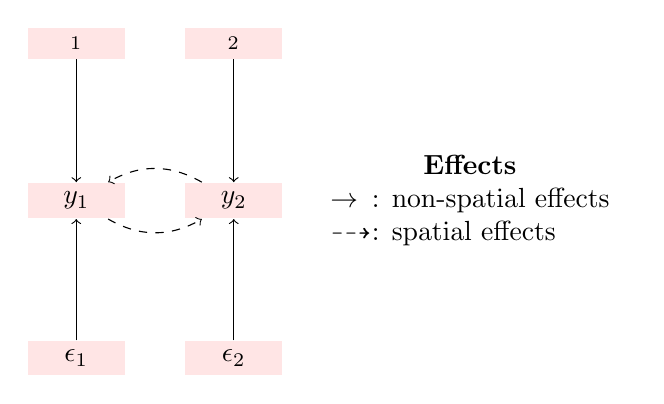
\begin{tikzpicture}
			\node[rectangle, text  width = 1cm, fill = red!10, align = center] (y1) at (-1,0) {$y_1$};
			\node[rectangle, text  width = 1cm, fill = red!10, align = center] (x1) at (-1,2) {$\vx_1$};
			\node[rectangle, text  width = 1cm, fill = red!10, align = center] (e1) at (-1,-2) {$\epsilon_1$};
			\node[rectangle, text  width = 1cm, fill = red!10, align = center] (y2) at (1, 0) {$y_2$};
			\node[rectangle, text  width = 1cm, fill = red!10, align = center] (x2) at (1,2) {$\vx_2$};
			\node[rectangle, text  width = 1cm, fill = red!10, align = center] (e2) at (1,-2) {$\epsilon_2$};
			
			\draw[->, solid] (x1) to (y1);
			\draw[->, solid] (x2) to (y2);
			\draw[->, solid] (e1) to (y1);
			\draw[->, solid] (e2) to (y2);
			\draw[dashed, ->] (y1) to[bend right] (y2);
			\draw[dashed, ->] (y2) to[bend right] (y1);

			% Legend
       \node (leyend) at (4, 0){
    \begin{tabular}{l@{: }l}
      \multicolumn{2}{c}{\textbf{Effects}}              \\
      $\rightarrow$                        & non-spatial effects    \\
      $\dashrightarrow$                     & spatial effects  \\
      \end{tabular}
      };
		\end{tikzpicture}
\end{figure}
\end{frame}

\begin{frame}
  \frametitle{Spatial Lag Model (SLM)}
  \begin{block}{}
  A full SLM specification with covariates in matrix form can be written as:

\begin{equation}\label{eq:Sar}
\vy  =  \alpha \vones_n+ \rho \mW\vy + \mX\vbeta + \epsilon,
\end{equation}
%
where $\vy$ is an $n\times 1$ vector of observations on the dependent variable, $\mX$ is an $n\times K$ matrix of observations on the explanatory variables, $\vbeta$ is the $K\times 1$ vector of parameters,  and $\vones_n$ is a $n\times 1$ vector of ones.
\end{block}

\begin{alertblock}{}
It is also important to find the \textbf{reduced form} of the process. 
\end{alertblock}
\end{frame}

\begin{frame}
  \frametitle{Reduce Form}
    \begin{alertblock}{}
    The \textbf{reduced form} of a system of equations is the result of solving the system for the \textbf{endogenous variables}. This gives the latter as functions of the exogenous variables, if any. For example, the general expression of a structural form is $f(\vy, \mX, \vepsi) = \vzeros$, whereas the reduced form of this model is given by $\vy = g(\mX, \vepsi)$, with $g$ as function. 
    \end{alertblock}
\end{frame}

\begin{frame}
  \frametitle{Reduce Form}
    
    \begin{eqnarray*}
     \vy &=& \rho \mW \vy + \mX\vbeta + \vepsi \\
     \vy &=& \left(\mI_n - \rho \mW\right)^{-1}\mX\vbeta + \left(\mI_n - \rho \mW\right)^{-1}\vepsi
    \end{eqnarray*}

  \begin{itemize}
    \item We need $\left(\mI_n - \rho \mW\right)$ to be \alert{invertible}. 
    \item From standard algebra theory: $\mA$ is invertible if $\det(\mA)\neq 0$
  \end{itemize}
\end{frame}

\begin{frame}
  \frametitle{Reduce Form}
  \begin{theorem}[Invertibility]
Let $\mW$ be a weighting matrix, such that $w_{ii} = 0$ for all $i = 1,...,n$, and assume that all of the roots of $\mW$ are real. Assume that $\mW$ is not row normalized. Let $\omega_{min}$ and $\omega_{max}$ be the minimum and maximum eigen value of $\mW$. Assume also that $\omega_{max} > 0$ and $\omega_{min} < 0$. Then $\left(\mI_n - \rho\mW\right)$ is nonsingular for all:

\begin{equation*}
  \omega_{min}^{-1} < \rho < \omega_{max}^{-1}
\end{equation*}
\end{theorem}
\end{frame}

%====================================================
\subsubsection{Reduced Form and Parameter Space}
%==================================================


\begin{frame}
  \frametitle{Reduce Form}
  
  \begin{block}{}
  Recall that for ease of interpretation, it is common practice to normalize $\mW$ such that the elements of each row sum to unity. Since $\mW$ is nonnegative, this ensures that all weights are between 0 and 1, and has the effect that the weighting operation can be interpreted as an averaging of neighboring values. 
  \end{block}
  
\begin{theorem}[Invertibility of Row-Normalized $\mW$ matrix]
If $\mW$ is row-normalized, then  $\left(\mI_n - \rho\mW\right)^{-1}$ exists for all $\left|\rho \right| < 1$
\end{theorem}
\end{frame}

\begin{frame}
  \frametitle{Reduce Form: Warning}
    \begin{alertblock}{}
      \alert{In spite of its popularity, row-normalized weighting has it drawbacks.} Row normalization alters the internal weighting structure of $\mW$ so that comparisons between rows become somewhat problematic.
    \end{alertblock}
    
    \begin{example}{}
    In view of this limitation, it is natural to consider simple scalar normalization which multiply $\mW$ by a single number, say $a \cdot \mW$, which removes any measure-unit effect but preserves relations between all rows of $\mW$. 
    \end{example}
\end{frame}

\begin{frame}
  \frametitle{Reduce Form: Other normalizations}
  In particular let

\begin{equation}
  \begin{aligned}
    a & = \min \left\lbrace r, c \right\rbrace \\
    r & = \max_i \sum_j \left|w_{ij}\right|\quad \mbox{maximal row sum of the absolute values} \\
    c & = \max_j \sum_i \left|w_{ij}\right|\quad \mbox{maximal column sum of the absolute values}.
  \end{aligned}
\end{equation}
\begin{itemize}
  \item Assuming that the elements of $\mW$ are nonegative, $(\mI_n - \rho\mW)$ will be nonsingular for all $\left|\rho\right| < 1/a$.
  \item This normalization has the advantage of ensuring that the resulting spatial weights, $w_{ij}$, are all between 0 and 1, and hence can still be interpreted as relative influence intensities.
\end{itemize}

\begin{alertblock}{}
This is an important result because a model which has a weighting matrix which is not row normalized can always be normalized in such a way that the inverse needed to solve the model will exists in an easily established region. 
\end{alertblock}
\end{frame}


%=================================================
\subsubsection{Expected Value and Variance}
%================================================

\begin{frame}
  \frametitle{Expected Value}
    The expectation is given by:

\begin{equation}\label{eq:expected_value_slm}
  \begin{aligned}
\E(\vy|\mX,\mW) & = \E\left[\left.\left(\mI_n - \rho \mW\right)^{-1}\left(\alpha \vones_n + \mX\vbeta\right) + \left(\mI_n - \rho \mW\right)^{-1}\vepsi\right|\mX,\mW\right] \\
                & = \left(\mI_n - \rho \mW\right)^{-1}\left(\alpha \vones_n + \mX\vbeta\right).
\end{aligned}
\end{equation}

To understand this expected value, we need to know the \textbf{Leontief Expansion}.
\end{frame}

\begin{frame}
  \frametitle{Expected Value}
  \begin{lemma}[Leontief Expansion]\label{lemma:Leontief}
If $\left|\rho\right|  < 1$, then
	\begin{equation*}
	(\mI - \rho \mW)^{-1} = \sum_{i = 0} ^{\infty}(\rho \mW)^{i}
	\end{equation*}
\end{lemma}

Then, using Lemma \ref{lemma:Leontief} (Leontief Expansion), the reduced mode can be written as:

\begin{equation}\label{eq:infinite_series_slm}
  \begin{aligned}
      \vy & = \left(\mI_n + \rho\mW + \rho^2\mW^2 + ...\right)\left(\alpha \vones_n + \mX\vbeta\right) + \left(\mI_n + \rho\mW + \rho^2\mW^2 + ...\right)\vepsi, \\
          & = \alpha\vones_n + \rho\mW\vones_n\alpha + \rho^2\mW^2\vones_n\alpha + ... + \mX\vbeta + \rho\mW\mX\vbeta + \rho^2\mW^2\mX\vbeta + ... \\
          & + \vepsi + \rho\mW\vepsi + \rho^2\mW^2\vepsi.
  \end{aligned}
\end{equation}
\end{frame}

\begin{frame}
  \frametitle{Expected Value}
  Expression (\ref{eq:infinite_series_slm}) can be simplified since the infinite series:

\begin{equation*}
\alpha\vones_n + \rho\mW\vones_n\alpha + \rho^2\mW^2\vones_\alpha + ... \to \frac{\vones_n\alpha}{\left(1 - \rho\right)},
\end{equation*}
%
since $\alpha$ is a scalar, the parameter $\left|\rho\right|  < 1$, and $\mW$ is row-stochastic. By definition $\mW\vones_n = \vones_n$ and therefore $\mW\mW\vones_n = \mW\vones_n = \vones$. Consequently, $\mW^l\vones_n = \vones_n$ for $l\geq 0$ (recall that $\mW^0 = \mI_n$). This allows to write:

\begin{equation*}
\vy = \frac{1}{(1-\rho)}\vones_n\alpha + \mX\vbeta + \rho\mW\mX\vbeta + \rho^2\mW^2\mX\vbeta + ... + \vepsi + \rho\mW\vepsi + \rho^2\mW^2\vepsi + ...
\end{equation*}

This expression allows defining two effects: a multiplier effect affecting the explanatory variables and a spatial diffusion effect affecting the error terms.
\end{frame}

\begin{frame}
  \frametitle{Variance-Covariance Matrix}
  From reduced-form Equation, we derive the variance-covariance matrix of $\vy$:

\begin{equation}
  \begin{aligned}
    \var\left(\left.\vy\right|\mW, \mX\right) & = \E\left(\left.\vy\vy^\top\right|\mW,\mX\right) \\ 
                               & = \left(\mI_n - \rho\mW\right)^{-1}\E\left(\left.\vepsi\vepsi^\top\right|\mW, \mX\right)\left(\mI_n- \rho\mW^\top\right)
  \end{aligned}
\end{equation}

\begin{itemize}
  \item This variance-covariance matrix is full, which implies that each location is correlated with every other location in the system (decreasing with the order of proximity).
  \item Moreover, the elements of the diagonal of $\E\left(\left.\vepsi\vepsi^\top\right|\mW, \mX\right)$ are not constant.
    \begin{itemize}
      \item This implies error heterokedasticity.
      \item Since we have not assumed anything about the error variance, we can say that $\E\left(\left.\vepsi\vepsi^\top\right|\mW, \mX\right)$ is a full matrix, say $\mOmega_{\epsilon}$.
      \item  This covers the possibility of heteroskedasticity, spatial autocorrelation, or both. In absence of either of these complications, the variance matrix simplifies to the usual $\sigma^2\mI_n$.
    \end{itemize}
\end{itemize}
\end{frame}

%=======================================
\subsection{Spatial Durbin Model}
%======================================

\begin{frame}
  \frametitle{Spatial Durbin Model (SDM)}
    The DGP is: 
    
    \begin{eqnarray*}
     \vy &=& \rho \mW \vy + \mX\vbeta + \mW\mX\vgamma + \vepsi \\
     \vy &=& \left(\mI_n - \rho \mW\right)^{-1}\left(\mX\vbeta + \mW\mX\vgamma\right) + \left(\mI_n - \rho \mW\right)^{-1}\vepsi 
    \end{eqnarray*}
\begin{block}{}  
  The SDM results in a spatial autoregressive model of a special form, including not only the spatially lagged dependent variable and the explanatory variables, but also the spatially lagged explanatory variables, $\mW\mX$: $\vy$ depends on own-regional factors from matrix $\mX$, plus the same factors averaged the $n$ neighboring regions.
\end{block}
\end{frame}


\begin{frame}
  \frametitle{Spatial Durbin Model (SDM)}
  \begin{figure}[ht]
	\centering
	\caption{The SDM for Two Regions}\label{figure:sdm}	
		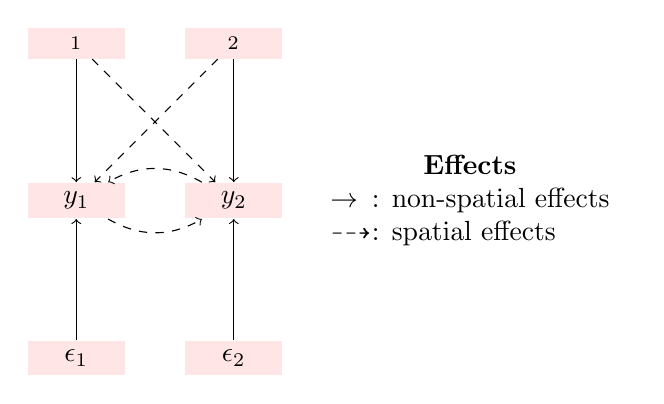
\begin{tikzpicture}
			\node[rectangle, text  width = 1cm, fill = red!10, align = center] (y1) at (-1,0) {$y_1$};
			\node[rectangle, text  width = 1cm, fill = red!10, align = center] (x1) at (-1,2) {$\vx_1$};
			\node[rectangle, text  width = 1cm, fill = red!10, align = center] (e1) at (-1,-2) {$\epsilon_1$};
			\node[rectangle, text  width = 1cm, fill = red!10, align = center] (y2) at (1, 0) {$y_2$};
			\node[rectangle, text  width = 1cm, fill = red!10, align = center] (x2) at (1,2) {$\vx_2$};
			\node[rectangle, text  width = 1cm, fill = red!10, align = center] (e2) at (1,-2) {$\epsilon_2$};

			\draw[->, solid] (x1) to (y1);
			\draw[->, solid] (x2) to (y2);
			\draw[->, solid] (e1) to (y1);
			\draw[->, solid] (e2) to (y2);
			\draw[dashed, ->] (y1) to[bend right] (y2);
			\draw[dashed, ->] (y2) to[bend right] (y1);
			\draw[dashed, ->] (x1) to (y2);
			\draw[dashed, ->] (x2) to (y1);
			%\draw[->, solid] (0,-4) to node[right, align = center] {$\sigma_i = 1$} (6,-5.4);
			%\draw[->, solid] (-6,-6.6) to node[right] {$\sigma_i = \sigma = 1$} (-2.5,-8);
			%\draw[->, solid] (6,-6.6) to node[right] {$\var(\veta_i)=\vzeros$} (2.5,-8);
			
			% Legend
       \node (leyend) at (4, 0){
    \begin{tabular}{l@{: }l}
      \multicolumn{2}{c}{\textbf{Effects}}              \\
      $\rightarrow$                        & non-spatial effects    \\
      $\dashrightarrow$                     & spatial effects  \\
      \end{tabular}
      };
		\end{tikzpicture}
\end{figure}
\end{frame}

%======================================
\subsection{Spatial Error Model}
%=======================================

\begin{frame}
  \frametitle{Spatial Error Model}
    We can also use spatial lags to reflect dependence in the disturbance process, which lead to the spatial error model (SEM):
    
    \begin{eqnarray*}
     \vy &=& \mX\vbeta + \vu \\
     \vu &=& \lambda\mW\vu + \vepsi \\
     \vy &=& \mX\vbeta + \left(\mI_n - \lambda \mW\right)^{-1}\vepsi 
    \end{eqnarray*}
    
  where $\lambda$ is the autoregressive parameter for the error lag $\mW\vu$ (to distinguish the notation from the spatial autoregressive coefficient $\rho$ in a spatial lag model), and $\vepsi$ is a generally a i.i.d noise.
\end{frame}

\begin{frame}
  \frametitle{Spatial Error Model}
  \begin{figure}[ht]
	\centering
	\caption{The SEM for Two Regions}\label{figure:sem}	
		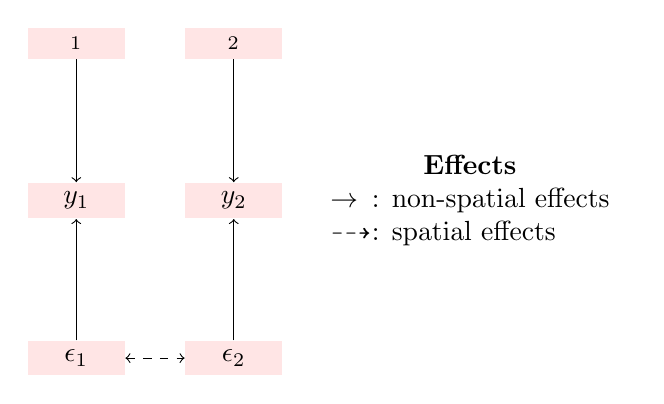
\begin{tikzpicture}
			\node[rectangle, text  width = 1cm, fill = red!10, align = center] (y1) at (-1,0) {$y_1$};
			\node[rectangle, text  width = 1cm, fill = red!10, align = center] (x1) at (-1,2) {$\vx_1$};
			\node[rectangle, text  width = 1cm, fill = red!10, align = center] (e1) at (-1,-2) {$\epsilon_1$};
			\node[rectangle, text  width = 1cm, fill = red!10, align = center] (y2) at (1, 0) {$y_2$};
			\node[rectangle, text  width = 1cm, fill = red!10, align = center] (x2) at (1,2) {$\vx_2$};
			\node[rectangle, text  width = 1cm, fill = red!10, align = center] (e2) at (1,-2) {$\epsilon_2$};

			\draw[->, solid] (x1) to (y1);
			\draw[->, solid] (x2) to (y2);
			\draw[->, solid] (e1) to (y1);
			\draw[->, solid] (e2) to (y2);
			\draw[dashed, <->] (e1) to (e2);

			% Legend
       \node (leyend) at (4, 0){
    \begin{tabular}{l@{: }l}
      \multicolumn{2}{c}{\textbf{Effects}}              \\
      $\rightarrow$                        & non-spatial effects    \\
      $\dashrightarrow$                     & spatial effects  \\
      \end{tabular}
      };
		\end{tikzpicture}
\end{figure}
\end{frame}

%==========================
\subsection{SAC}
%===========================

\begin{frame}
  \frametitle{Spatial Autocorrelation Model (SAC)}
  
  This model contains spatial dependence in both the dependent variable and the disturbances:
  
      \begin{eqnarray*}
     \vy &=& \rho \mW \vy + \mX\vbeta + \vu \\
     \vu &=& \lambda\mM\vu + \vepsi \\
     \vy & = & \left(\mI_n - \rho \mW\right)^{-1}\mX\vbeta + \left(\mI_n - \rho \mW\right)^{-1}\left(\mI_n - \rho \mM\right)^{-1}\vepsi
    \end{eqnarray*}
    
    where $\mW$ may be set equal to $\mM$
\end{frame}


\begin{frame}[fragile]
  \frametitle{Elhorts' taxonomy}
\begin{adjustbox}{max totalsize={.9\textwidth}{.7\textheight},center}
\begin{tikzpicture}[scale = 0.8]
			\node[rectangle, text  width = 5cm, fill = red!10, align = center] (gns) at (0,0) {\scriptsize General nesting spatial model \\
			\begin{eqnarray*}
			\vy &=& \rho\mW\vy + \mX\vbeta + \mW\mX\vgamma + \vu \\
			\vu &=& \lambda\mW\vu + \vepsi
			\end{eqnarray*}};
			
			\node[rectangle, text  width = 3cm, fill = red!10, align = center] (sac) at (6,4) {\scriptsize  SAC \\
			\begin{eqnarray*}
			\vy &=& \rho\mW\vy + \mX\vbeta + \vu \\
			\vu &=& \lambda\mW\vu + \vepsi
			\end{eqnarray*}};
			
			\node[rectangle, text  width = 3cm, fill = red!10, align = center] (sdm) at (6,0) {\scriptsize  Spatial durbin model \\
			\begin{equation*}
			\vy = \rho\mW\vy + \mX\vbeta + \mW\mX\vgamma + \vepsi
			\end{equation*}};
			
			\node[rectangle, text  width = 3cm, fill = red!10, align = center] (sde) at (6,-4) {\scriptsize Spatial durbin error model \\
			\begin{eqnarray*}
			\vy &=& \mX\vbeta + \mW\mX\vgamma + \vu \\
			\vu &=& \lambda\mW\vu + \vepsi
			\end{eqnarray*}};
			
			\node[rectangle, text  width = 3cm, fill = red!10, align = center] (slm) at (12,4) {\scriptsize Spatial Lag Model \\
			\begin{equation*}
			\vy = \rho\mW\vy + \mX\vbeta + \vepsi
			\end{equation*}};
			
			\node[rectangle, text  width = 3cm, fill = red!10, align = center] (slx) at (12,0) {\scriptsize SLX \\
			\begin{equation*}
			\vy = \mX\vbeta + \mW\mX\vgamma + \vepsi
			\end{equation*}};
			
			\node[rectangle, text  width = 3cm, fill = red!10, align = center] (sem) at (12,-4) {\scriptsize Spatial error model \\
			\begin{eqnarray*}
			\vy &=& \mX\vbeta + \vu \\
			\vu &=& \lambda\mW\vu + \vepsi
			\end{eqnarray*}};
			
			\node[rectangle, text  width = 2cm, fill = red!10, align = center] (ols) at (16,0) {\scriptsize OLS \\
			\begin{equation*}
			\vy = \mX\vbeta + \vepsi
			\end{equation*}};

			\draw (gns) -- (sac) node [->, solid, midway, above, sloped] {\scriptsize $\vgamma = 0$};
			\draw (gns) -- (sdm) node [->, solid, midway, above, sloped] {\scriptsize $\lambda = 0$};
			\draw (gns) -- (sde) node [->, solid, midway, above, sloped] {\scriptsize $\rho = 0$};
			\draw (sac) -- (slm) node [->, solid, midway, above, sloped] {\scriptsize $\lambda = 0$};
			\draw (sac) -- (sem) node [->, solid, near end, above, sloped] {\scriptsize $\rho = 0$};
			\draw (sdm) -- (slx) node [->, solid, near end, above, sloped] {\scriptsize $\rho = 0$};
			\draw (sde) -- (slx) node [->, solid, near start, above, sloped] {\scriptsize $\lambda = 0$};
			\draw (sdm) -- (slm) node [->, solid, midway, above, sloped] {\scriptsize $\gamma = 0$};
			\draw (sdm) -- (sem) node [->, solid, midway, above, sloped] {\scriptsize $\gamma = -\rho\beta$};
			\draw (sde) -- (sem) node [->, solid, midway, above, sloped] {\scriptsize $\gamma = 0$};
			\draw (slm) -- (ols) node [->, solid, midway, above, sloped] {\scriptsize $\rho = 0$};
			\draw (slx) -- (ols) node [->, solid, midway, above, sloped] {\scriptsize $\gamma = 0$};
			\draw (sem) -- (ols) node [->, solid, midway, above, sloped] {\scriptsize $\lambda = 0$};
			%\draw[->, solid] (x2) to (y2);
			%\draw[->, solid] (e1) to (y1);
			%\draw[->, solid] (e2) to (y2);
			%\draw[dashed, <->] (e1) to (e2);

			% Legend
     %  \node (leyend) at (4, 0){
    %     \begin{tabular}{l@{: }l}
    %  \multicolumn{2}{c}{\textbf{Effects}}              \\
    %  $\rightarrow$                        & non-spatial effects    \\
    %  $\dashrightarrow$                     & spatial effects  \\
    %  \end{tabular}
    %  };
\end{tikzpicture}
\end{adjustbox}
\end{frame}

%***********************************************
\section{Motivating Spatial Models}
%***********************************************

\subsection{SLM as a Long-run Equilibrium}

\begin{frame}
  \frametitle{Long-run Equilibrium}
  Consider the following:
    \begin{itemize}
      \item $\vy_t$: dependent variable vector at time $t$.
      \item $\mW\vy_t$: time lag of the average neighboring values of the dependent variable observed during previous period. 
      \item $\mX_t= \mX$: characteristics of regions remain relatively fixed over time.
    \end{itemize}
    
    Then, the more appropriate process is the following:

\begin{equation}\label{eq:slm_with_time}
\vy_t = \rho \mW\vy_{t-1} + \mX\vbeta + \vepsi_t.
\end{equation}

Note that we can replace $\vy_{t-1}$ on the right-hand side of (\ref{eq:slm_with_time}) with:

\begin{equation*}
\vy_{t-1} = \rho \mW\vy_{t-2} + \mX\vbeta + \vepsi_{t-1},
\end{equation*}
%
producing:

\begin{eqnarray}
y_t & = & \mX\vbeta +\rho\mW\left(\mX\vbeta + \rho \mW\vy_{t-2} + \vepsi_{t-1}\right) + \vepsi_t, \label{eq:recur_1}\\
&=& \mX\vbeta +\rho\mW\mX\vbeta + \rho^2\mW^2\vy_{t-2} + \epsilon_t + \rho\mW\vepsi_{t-1}.\label{eq:recur_2}
\end{eqnarray}
\end{frame}


\begin{frame}
  \frametitle{Long-run Equilibrium}
    Recursive substitution for past values of the vector $\vy_{t-r}$ on the right-hand side of (\ref{eq:recur_2}) over $q$ periods leads to:

\begin{equation*}
  \begin{aligned}
    \vy_t &= \left(\mI_n + \rho\mW + \rho^2\mW^2 + ... + \rho^{q-1}\mW^{q-1}\right)\mX\vbeta + \rho^q\mW^q\vy_{t-q} + \vu,\\
    \vu = & = \vepsi_{t} + \rho\mW\vepsi_{t-1} + \rho^2\mW^2\vepsi_{t-2} + ... + \rho^{q-1}\mW^{q-1}\vepsi_{t - (q-1)}. 
  \end{aligned}
\end{equation*}

Noting that:

\begin{equation}\label{eq:expectation_time}
  \mE\left(\vy_t\right) = \left(\mI_n + \rho\mW + \rho^2\mW^2 + ... + \rho^{q-1}\mW^{q-1}\right)\mX\vbeta + \rho^q\mW^q\vy_{t-q},
\end{equation}
%
where we use the fact that $\E(\vepsi_{t-r}) = 0, r = 0, ..., q-1$, which also implies that $\E(\vu) = \vzeros$.
\end{frame}


\begin{frame}
  \frametitle{Long-run Equilibrium}
  finally, taking the limit of (\ref{eq:expectation_time}), 


\begin{equation}\label{eq:steady_state}
\lim_{q\to \infty} \mE\left(\vy_t\right) = \left(\mI_n - \rho\mW\right)^{-1}\mX\vbeta.
\end{equation}
%
Note that we use the fact that the magnitude of $\rho^q\mW^q\vy_{t-q}$ tends to zero for large $q$, under the assumption that $\lvert \rho \rvert <1$ and assuming that $\mW$ is row-stochastic, so the matrix $\mW$ has a principal eigenvalue of 1. 

\begin{alertblock}{Key point:}
Equation (\ref{eq:steady_state}) states that we can interpret the observed cross-sectional relation as the outcome or expectation of a long-run equilibrium or steady state. Note that this provides a dynamic motivation for the data generating process of the cross-sectional SLM that serves as a \textbf{workhorse} of spatial regression modeling. That is, a cross-sectional SLM relation can arise from time-dependence of decisions by economic agents located at various point in space when decisions depend on those neighbors. 
\end{alertblock}
\end{frame}


\subsection{SEM and Omitted Variables Motivation}

\begin{frame}
  \frametitle{SEM and Omitted Variables Motivation}
  Consider the following process:

\begin{equation*}
\vy = \vx\beta + \vz\theta,
\end{equation*}
%
where $\vx$ and $\vz$ are \textbf{uncorrelated} vectors of dimension $n\times 1$, and the vector $\vz$ follows the following spatial autoregressive process:

\begin{eqnarray*}
  \vz &=& \rho \mW\vz + \vr \\
  \vz &=& \left(\mI_n - \rho\mW\right)^{-1}\vr
\end{eqnarray*}
%
where $\vr \sim \rN(0, \sigma^2_{\epsilon}\mI_n)$. Examples of $\vz$ are culture, social capital, neighborhood prestige. 

If $\vz$ is not observed, then:


\begin{equation}\label{eq:sem_omited_moti}
  \begin{aligned}
    \vy & = \vx\beta + \vu \\
    \vu & = \left(\mI_n - \rho\mW\right)^{-1}\vepsi
  \end{aligned}
\end{equation}
%
where $\vepsi = \theta\vr$. Then, we have the DGP for the spatial error model.
\end{frame}

\subsection{SDM and Omitted Variables Motivation}

\begin{frame}
  \frametitle{SDM and Omitted Variables Motivation}
    Now suppose that $\mX$ and $\vepsi$ from (\ref{eq:sem_omited_moti}) are correlated, given by the following process:

\begin{equation}\label{eq:cor_x_epsi}
\begin{aligned}
  \vepsi & = \vx \gamma + \vv \\
  \vv    & \sim \rN(0, \sigma^2\mI_n) 
\end{aligned}
\end{equation}
%
where the scalar parameters $\gamma$ and $\sigma^2$ govern the strength of the relationship between $\mX$ and $\vz = (\mI_n-\rho\mW)^{-1}\vr$. Inserting (\ref{eq:cor_x_epsi}) into (\ref{eq:sem_omited_moti}), we obtain:

\begin{equation}
  \begin{aligned}
    \vy & = \vx\beta + \left(\mI_n - \rho\mW\right)^{-1}\vepsi \\
        & = \vx\beta + \left(\mI_n - \rho\mW\right)^{-1}\left(\vx \gamma + \vv\right) \\
        & = \vx\beta + \left(\mI_n - \rho\mW\right)^{-1}\vx \gamma + \left(\mI_n - \rho\mW\right)^{-1}\vv \\
       \left(\mI_n - \rho\mW\right)\vy & = \left(\mI_n - \rho\mW\right)\vx\beta  + \vv \\
       \vy & = \rho\mW\vy + \vx\left(\beta + \gamma\right) + \mW\vx(-\rho\beta) + \vv
  \end{aligned}
\end{equation}

This is the Spatial Durbin Model (SDM), which includes a spatial lag of the dependent variable $\vy$, as well as the explanatory variables $\vx$
\end{frame}




%***********************************************
\section{Interpreting Spatial Models}
%***********************************************

\subsection{Measuring Spillovers}

\begin{frame}
  \frametitle{Global and local spillovers}
  \textbf{\alert{Spillovers:} Key in Regional Science.}
  
  \begin{alertblock}{Spillovers}
   A basic definition of spillovers in a spatial context would be that changes occurring in one region exert impacts on other regions
  \end{alertblock}

\begin{itemize}
  \item Changes in tax rate by one spatial unit might exert an impact on tax rate setting decisions of nearby regions, a phenomenon that has been labeled tax mimicking and yardstick competition between local government (see our example below). 
  \item Situations where home improvements made by one homeowner exert a beneficial impact on selling prices of neighboring homes.
  \item Innovation by university researchers diffuses to nearby firms.
  \item Air or water pollution generated in one region spills over to nearby regions. 
\end{itemize}

\end{frame}


\begin{frame}
  \frametitle{Global and local spillovers}
    \begin{definition}[Global Spillovers]
	 Global spillovers arise when changes in a characteristic of one region impact all regions' outcomes. This applies even to the region itself since impacts can pass to the neighbors and back to the own region (feedback). Specifically, global spillovers impact the neighbors, neighbors to the neighbors, neighbors to the neighbors to the neighbors and so on. 
\end{definition}

The endogenous interactions produced by global spillovers lead to a scenario where changes in one region set in motion a sequence of adjustments in (potentially) all regions in the sample such that a new long-run steady state equilibrium arises.
\end{frame}

\begin{frame}
  \frametitle{Global and local spillovers}
   \begin{definition}[Local Spillovers]
 	Local spillovers represent a situation where the impact fall only on nearby or immediate neighbors, dying out before they impact regions that are neighbors to the neighbors.
 \end{definition}	

The main difference is that feedback or endogenous interaction is only  possible for global spillovers.
\end{frame}

\begin{frame}
  \frametitle{Marginal Effects}
    \begin{itemize}
      \item Mathematically, the notion of spillover can be thought as the derivative $\partial y_i/ \partial x_j$. This means that changes to explanatory variables in region $i$ impact the dependent variable in region $j\neq i$.
      \item In the OLS model we have $\partial y_i/ \partial x_j = 0$
    \end{itemize}
\end{frame}

\begin{frame}
  \frametitle{Measuring spillovers}
    Consider the SDM model, which can be re-written as:


\begin{equation}
\begin{aligned}
(\mI_n - \rho\mW)\vy & = \mX\vbeta + \mW\mX\vtheta + \vepsi \\
\vy & =   \sum_{r=1}^k\mS_r(\mW)\vx_r + \mA(\mW)^{-1}\vepsi
\end{aligned}
\end{equation}

where $\mS_r = \mA(\mW)^{-1}\left(\mI_n\beta_r + \mW\theta_r\right)$, and

\begin{equation*}
 \vx_r = \begin{pmatrix}
          x_{r1} \\
          x_{r2} \\
          \vdots \\
          x_{rn}
        \end{pmatrix}
\end{equation*}
\end{frame}


\begin{frame}
  \frametitle{Measuring spillovers}
  Now, consider the expansion of the expected value:


\begin{equation}
\begin{pmatrix}
\E(y_1) \\ \E(y_2) \\ \vdots \\ \E(y_n)
\end{pmatrix}
=
\sum_{r=1}^k\begin{pmatrix}
S_r(\mW)_{11} & S_r(\mW)_{12} & \hdots & S_r(\mW)_{1n} \\
S_r(\mW)_{21} & S_r(\mW)_{22} & \hdots & S_r(\mW)_{2n} \\
\vdots & \vdots & \ddots & \vdots \\ 
S_r(\mW)_{n1} & S_r(\mW)_{n2} & \hdots & S_r(\mW)_{nn} 
\end{pmatrix}
\begin{pmatrix}
x_{1r} \\ x_{2r} \\ \vdots \\ x_{nr} 
\end{pmatrix}
\end{equation}

For a single dependent variable, this would be:


\begin{equation}
\E(y_i) = \sum_{r=1}^k\left[S_r(\mW)_{i1}x_{1r} + ... + S_r(\mW)_{n1}x_{nr}\right]
\end{equation}
\end{frame}


\begin{frame}
\frametitle{Measuring spillovers}

\begin{enumerate}
  \item Indirect effects: The impact on the expected value of location $i$ given a change in the explanatory variable $x_k$ in location $j$ is 

\begin{equation}
\frac{\partial \E(y_i)}{\partial x_{jr}} = S_r(\mW)_{ij}
\end{equation}

where $S_r(\mW)_{ij}$ is this equation represents the $i,j$th element of the matrix $\mS_r(\mW)$.

\item Direct effects: The impact of the expected value of region $i$, given a change in certain variable for the same region is given by

\begin{equation}
\frac{\partial \E(y_i)}{\partial x_{ir}} = S_r(\mW)_{ii}
\end{equation}

This impact includes the \textbf{effect of feedback loops} where observation $i$ affects observation $j$ and observation $j$ also affects observation $i$: a change in $x_{ir}$ will affect the expected value of dependent variable in $i$, then will pass through the neighbors of $i$ and back to the region itself.
\end{enumerate}
\end{frame}

\begin{frame}
\frametitle{Measuring spillovers}
Let us write the all the marginal effects in matrix notation as follows:


\begin{equation*}\label{eq:matrix_marginal_effects}
\begin{aligned}
 \underset{n \times n}{\begin{pmatrix}
  \frac{\partial \E(\vy)}{\partial x_{1r}} & \frac{\partial \E(\vy)}{\partial x_{2r}} & \hdots & \frac{\partial \E(\vy)}{\partial x_{nr}} 
   \end{pmatrix}} & = 
  \begin{pmatrix}
  \frac{\partial \E(y_1)}{\partial x_{1r}} & \frac{\partial \E(y_1)}{\partial x_{2r}} & \hdots & \frac{\partial \E(y_1)}{\partial x_{nr}} \\
  \frac{\partial \E(y_2)}{\partial x_{1r}} & \frac{\partial \E(y_2)}{\partial x_{2r}} & \hdots & \frac{\partial \E(y_2)}{\partial x_{nr}} \\
  \vdots & \vdots & \ddots & \vdots \\
  \frac{\partial \E(y_n)}{\partial x_{1r}} & \frac{\partial \E(y_n)}{\partial x_{2r}} & \hdots & \frac{\partial \E(y_n)}{\partial x_{nr}} 
  \end{pmatrix} \\
  & = \mA(\mW)^{-1}\left(\mI_n\beta_r + \mW\theta_r\right) = \mS_r(\mW) \\
  & = (\mI_n - \rho\mW)^{-1}
  \begin{pmatrix}
    \beta_r  & w_{12} \theta_r  & \hdots & w_{1n}\theta_r \\
    w_{21} \theta_r  & \beta_r   & \hdots & w_{2n}\theta_r \\
    \vdots & \vdots & \ddots & \vdots \\
    w_{n1} \theta_r  & w_{n2} \theta_r  & \hdots  & \beta_r \\
  \end{pmatrix}
\end{aligned}  
\end{equation*}
\end{frame}

\begin{frame}
\frametitle{Measuring spillovers}

Following Elhorst (2010), consider:

\begin{equation}\label{eq:w_mat_ex_spill}
  \mW = \begin{pmatrix}
          0      & 1 & 0 \\
          w_{21} & 0 & w_{23} \\
          0      & 1 & 0
        \end{pmatrix}
\end{equation}

and


\begin{equation}\label{eq:w_Imat_ex_spill}
  \mA(\mW)^{-1} = \frac{1}{1 - \rho^2}
  \begin{pmatrix}
          1 - w_{23}\rho^2     & \rho & \rho^2 w_{23}\\
          \rho w_{21} & 1 & \rho w_{23} \\
          \rho^2 w_{21}      & \rho & 1 - w_{21}\rho^2 
        \end{pmatrix}
\end{equation}


Substituting Equations \ref{eq:w_mat_ex_spill} and \ref{eq:w_Imat_ex_spill} into Equation \ref{eq:matrix_marginal_effects} we get:

\tiny
\begin{equation*}
\begin{split}
  \begin{pmatrix}
  \frac{\partial \E(\vy)}{\partial x_{1r}} & \frac{\partial \E(\vy)}{\partial x_{2r}} & \hdots & \frac{\partial \E(\vy)}{\partial x_{nr}} 
   \end{pmatrix} & = \frac{1}{1 - \rho^2} \\
   & \begin{pmatrix}
    \left(1 -  w_{23}\rho^2\right)\beta_r + \left(w_{21}\rho\right) \theta_r & \rho \beta_r + \theta_r & \left(w_{23}\rho^2\right)\beta_r + (\rho w_{23})\theta_r \\
    (w_{21}\rho)\beta_r + w_{21}\theta_r & \beta_r + \rho \theta_r & (w_{23}\rho)\beta_r + w_{23}\theta_r \\
    (w_{21}\rho^2)\beta_r + (w_{21}\rho)\theta_r & \rho \beta_r + \theta_r & (1 -  w_{21}\rho^2)\beta_r + (w_{23}\rho)\theta_r
   \end{pmatrix}
   \end{split}
\end{equation*}
\end{frame}


\begin{frame}
    \frametitle{Measuring spillovers}
    \begin{itemize}
      \item Note that direct effects =  diagonal of previous matrix. 
      \item Indirect effects = every non-diagonal elements.
        \begin{itemize}
          \item What happens with the IEs if $\rho = 0$ and $\theta_r = 0$?
        \end{itemize}
      \item The direct and indirect effects are different for different units in the sample. 
      \item IEs that occur if $\theta_r \neq 0$ are known as \alert{local effects}, as opposed to IE that occurs if $\rho \neq 0$ and that are known as \alert{global effects}.
        \begin{itemize}
          \item Local  effects: If the element $w_{ij}$ is non-zero (zero), then the effect of $x_{jk}$ on $y_i$ is also non-zero (zero). Note that:
              \begin{equation*}
                \frac{\partial \E(y_3)}{\partial x_{1r}} = \frac{1}{1 - \rho^2}\left(w_{21}\rho^2\beta_r + w_{21}\rho\theta_r\right)
              \end{equation*}
              
              therefore, the impact of $x_{1r}$ on $y_3$ will depend on the global effect $(w_{21}\rho^2 \beta_r)/(1 - \rho^2)$ and the local effect $w_{21}\rho\theta_r / (1 - \rho^2)$
          \item What if $w_{21}=0$? what if $\rho$ increases?
        \end{itemize}
    \end{itemize}
\end{frame}


\begin{frame}{Summary Measures}
  \begin{itemize}
    \item It can be noted that the change of each variable in each region implies $n^2$ potential marginal effects.  
    \item If we have $K$ variables in our model, this implies $K\times n^2$ potential measures.
    \item Even for small values of $n$ and $K$, it may already be rather difficult to report these results compactly
  \end{itemize}
  \begin{alertblock}{}
    We need summary measures!
  \end{alertblock}
\end{frame}

\begin{frame}{Summary Measures}
\begin{definition}[Average Direct Impact]\label{def:ADI}
Let $\mS_r = \mA(\mW)^{-1}\left(\mI_n\beta_r + \mW\theta_r\right)$ for variable $r$. The impact of changes in the $i$th observation of $x_r$, which is denoted $x_{ir}$, on $y_i$ could be summarized by measuring the average $S_r(\mW)_{ii}$, which equals
	
	\begin{equation}
		\mbox{ADI} = \frac{1}{n}\tr\left(\mS_r(\mW)\right)
	\end{equation}
\end{definition}
Averaging over the direct impact associated with all observations $i$ is similar in spirit to typical regression coefficient interpretations that represent average response of the dependent to independent variables over the sample of observations. 	
\end{frame}

\begin{frame}{Summary Measures}
\begin{definition}[Average Total Impact to an Observation]\label{def:ATIT}
	Let $\mS_r = \mA(\mW)^{-1}\left(\mI_n\beta_r + \mW\theta_r\right)$ for variable $r$. The sum across the $i$th row of $\mS_r(\mW)$ would be represent the total impact on individual observation $y_i$ resulting from changing the $r$th explanatory variable by the same amount across all $n$ observations. There are $n$ of these sums given by the column vector $\vc_r = \mS_r(\mW)\vones_n$, so an average of these total impacts is:
		\begin{equation}
		\mbox{ATIT} = \frac{1}{n} \vones_n'\vc_r
		\end{equation} 
\end{definition}
\begin{definition}[Average Total Impact from an Observation]\label{def:ATIF}
	Let $\mS_r = \mA(\mW)^{-1}\left(\mI_n\beta_r + \mW\theta_r\right)$ for variable $r$. The sum down the $j$th column of $\mS_r(\mW)$ would yield the total impact over all $y_i$ from changing the $r$th explanatory variable by an amount in the $j$th observation. There are $n$ of these sums given by the row vector $\vr_r = \vones_n'\mS_{r}(\mW)$, so an average of these total impacts is:
				\begin{equation}
				\mbox{ATIF} = \frac{1}{n} \vr_r\vones_n
				\end{equation} 
\end{definition}
\end{frame}

\begin{frame}
    \frametitle{Reporting Direct and Indirect Effects}
We might compute the following measures representing the average total impacts, the average direct impacts, and the average indirect impacts from changes in the model variable $X_r$
        
        \begin{eqnarray*}
          \bar{M}(r)_{\mbox{direct}} &=& n^{-1}\tr(S_r(W)) \\
          \bar{M}(r)_{\mbox{total}}  &=& n^{-1}\vones'S_r(W)\vones \\
          \bar{M}(r)_{\mbox{indirect}} &=& \bar{M}(r)_{\mbox{total}}  - \bar{M}(r)_{\mbox{direct}} 
        \end{eqnarray*}
        
These measures are \textbf{inefficient} since we require inversion of the $n\times n$ matrix $(\mI_n - \rho \mW)$.
\end{frame}

\begin{frame}
    \frametitle{Reporting Direct and Indirect Effects}
      \alert{Remark} These effects reflect how these changes would work through the simultaneous dependence system over time to culminate in a new steady state equilibrium!
\end{frame}

%=====================
\subsection{Partitioning Global Effects Estimates Over Space}
%======================

\begin{frame}
    \frametitle{Reporting Direct and Indirect Effects}
    \begin{itemize}
      \item These scalar summary measures of impact reflect how these changes would work thought the simultaneous dependence system over time to culminate in a new steady state equilibrium. 
      \item Impacts that would take place once all regions reach their equilibrium after the initial change in the variable of interest. 
      \item However one could track the cumulative effects as the impacts pass through neighbors, neighbors of neighbors and so on. 
    \end{itemize}
    
\begin{equation}
  \begin{pmatrix}
  \frac{\partial \E(\vy)}{\partial x_{1r}} & \frac{\partial \E(\vy)}{\partial x_{2r}} & \hdots & \frac{\partial \E(\vy)}{\partial x_{nr}} 
   \end{pmatrix} \approx \left(\mI_n  + \rho \mW + \rho^2\mW^2 + \rho^3\mW^3 + ... + \rho^l\mW^l\right)\mI_n\beta_r  
\end{equation}
    
This expression allow us to observe the impact associated with each power of $\mW$, where these powers corresponds to the observation themselves (zero-order), immediate neighbors (first-order), neighbors of neighbors (second-order), and so on. Using this expansion we could account for both the cumulative effects as marginal and total direct, indirect associated with different order of neighbors.
\end{frame}


\subsection{Lesage's Book Example}



\begin{frame}
  \frametitle{Lesage's Example of Spillovers}
\begin{figure}
     \centering
     \begin{subfigure}[b]{0.49\columnwidth}
         \centering
         
\includegraphics[height=5cm, width=\linewidth]{James_Lesage}
         \caption{Professor James Lesage}
     \end{subfigure}
     \hfill
     \begin{subfigure}[b]{0.4\columnwidth}
         \centering
         
\includegraphics[height=5cm, width=\linewidth]{Pace}
         \caption{Professor R Kelley Pace}
     \end{subfigure}
        \caption{Introduction to Spatial Econometrics}
\end{figure}
\end{frame}


\begin{frame}
  \frametitle{Lesage's Example of Spillovers}
   Consider the following example,
     	\begin{figure}[H]
		    \centering 
		      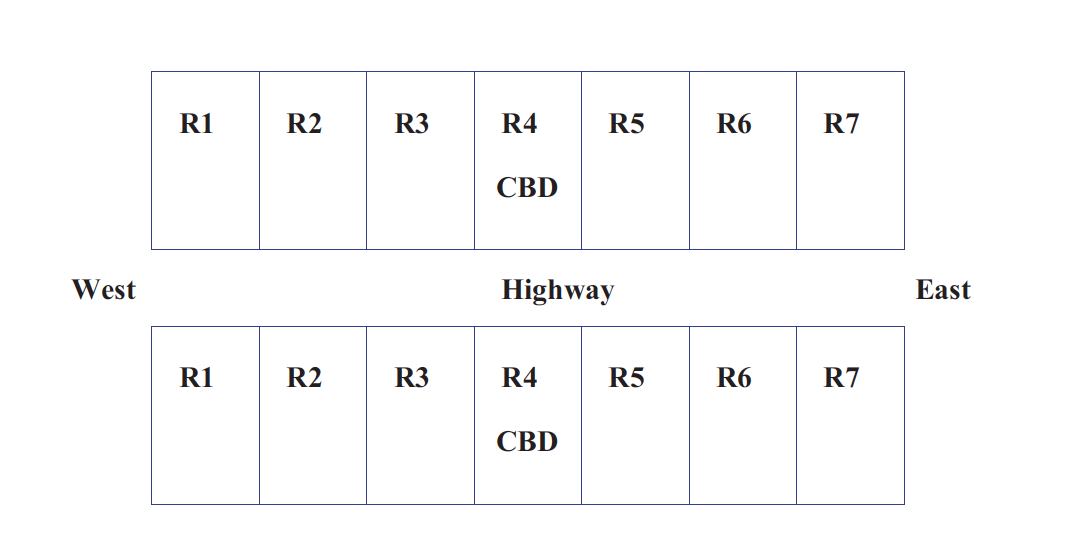
\includegraphics[width = 8cm, height=6cm]{Lesage_ex.png}
	    \end{figure}
\end{frame}

\begin{frame}
  \frametitle{Lesage's Example of Spillovers}
   Consider the following example,
     	\begin{figure}[H]
		    \centering 
		      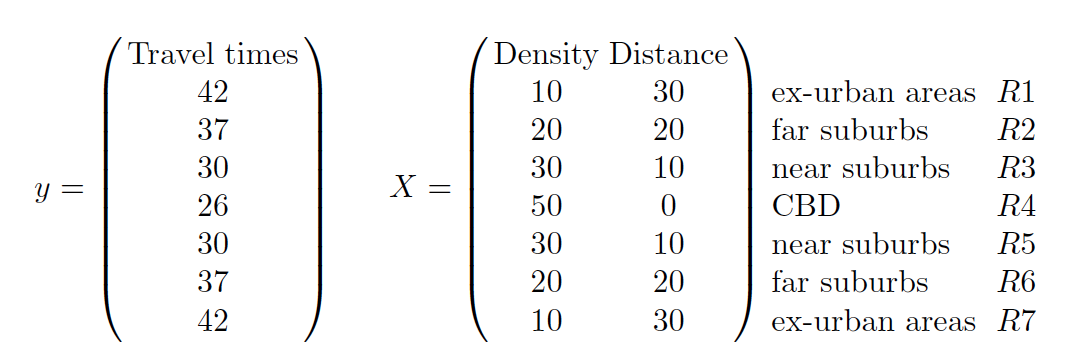
\includegraphics[width = 8cm, height=4cm]{Lesage_ex2.png}
	    \end{figure}
\end{frame}

\begin{frame}
  \frametitle{Lesage's Example of Spillovers}
    \begin{itemize}
      \item Consider 
        \begin{equation}
          \vy = \rho\mW\vy + \mX\vbeta + \vepsi
        \end{equation}
        
        such that:
        
        \begin{equation}
          \widehat{\vy} = (\mI_n - \widehat{\rho}\mW)^{-1}\mX\widehat{\vbeta}
        \end{equation}
        
      \item Somehow, we get the following estimates:
        \begin{itemize}
          \item $\widehat{\vbeta} = (0.135 \quad 0.561)'$
          \item $\widehat{\rho} = 0.642$. It indicates positive spatial dependence in the commuting times. 
        \end{itemize}
      \item What would happen if we double the density of region 2?  
    \end{itemize}
\end{frame}


\begin{frame}[fragile]
  \frametitle{Lesage's Example of Spillovers}
\begin{knitrout}\small
\definecolor{shadecolor}{rgb}{0.969, 0.969, 0.969}\color{fgcolor}\begin{kframe}
\begin{alltt}
\hlcom{# Estimated coefficients}
\hldef{b} \hlkwb{<-} \hlkwd{c}\hldef{(}\hlnum{0.135}\hldef{,} \hlnum{0.561}\hldef{)}
\hldef{rho} \hlkwb{<-} \hlnum{0.642}

\hlcom{# W and X}
\hldef{X} \hlkwb{<-} \hlkwd{cbind}\hldef{(}\hlkwd{c}\hldef{(}\hlnum{10}\hldef{,} \hlnum{20}\hldef{,} \hlnum{30}\hldef{,} \hlnum{50}\hldef{,} \hlnum{30}\hldef{,} \hlnum{20}\hldef{,} \hlnum{10}\hldef{),}
         \hlkwd{c}\hldef{(}\hlnum{30}\hldef{,} \hlnum{20}\hldef{,} \hlnum{10}\hldef{,} \hlnum{0}\hldef{,} \hlnum{10}\hldef{,} \hlnum{20}\hldef{,} \hlnum{30}\hldef{))}
\hldef{W} \hlkwb{<-} \hlkwd{cbind}\hldef{(}\hlkwd{c}\hldef{(}\hlnum{0}\hldef{,} \hlnum{1}\hldef{,} \hlnum{0}\hldef{,} \hlnum{0}\hldef{,} \hlnum{0}\hldef{,} \hlnum{0}\hldef{,} \hlnum{0}\hldef{),}
         \hlkwd{c}\hldef{(}\hlnum{1}\hldef{,} \hlnum{0}\hldef{,} \hlnum{1}\hldef{,} \hlnum{0}\hldef{,} \hlnum{0}\hldef{,} \hlnum{0}\hldef{,} \hlnum{0}\hldef{),}
         \hlkwd{c}\hldef{(}\hlnum{0}\hldef{,} \hlnum{1}\hldef{,} \hlnum{0}\hldef{,} \hlnum{1}\hldef{,} \hlnum{0}\hldef{,} \hlnum{0}\hldef{,} \hlnum{0}\hldef{),}
         \hlkwd{c}\hldef{(}\hlnum{0}\hldef{,} \hlnum{0}\hldef{,} \hlnum{1}\hldef{,} \hlnum{0}\hldef{,} \hlnum{1}\hldef{,} \hlnum{0}\hldef{,} \hlnum{0}\hldef{),}
         \hlkwd{c}\hldef{(}\hlnum{0}\hldef{,} \hlnum{0}\hldef{,} \hlnum{0}\hldef{,} \hlnum{1}\hldef{,} \hlnum{0}\hldef{,} \hlnum{1}\hldef{,} \hlnum{0}\hldef{),}
         \hlkwd{c}\hldef{(}\hlnum{0}\hldef{,} \hlnum{0}\hldef{,} \hlnum{0}\hldef{,} \hlnum{0}\hldef{,} \hlnum{1}\hldef{,} \hlnum{0}\hldef{,} \hlnum{1}\hldef{),}
         \hlkwd{c}\hldef{(}\hlnum{0}\hldef{,} \hlnum{0}\hldef{,} \hlnum{0}\hldef{,} \hlnum{0}\hldef{,} \hlnum{0}\hldef{,} \hlnum{1}\hldef{,} \hlnum{0}\hldef{))}
\hldef{Ws} \hlkwb{<-} \hldef{W} \hlopt{/} \hlkwd{rowSums}\hldef{(W)}
\hlcom{# Prediction}
\hldef{yhat_1} \hlkwb{<-} \hlkwd{solve}\hldef{(}\hlkwd{diag}\hldef{(}\hlkwd{nrow}\hldef{(W))} \hlopt{-}  \hldef{rho} \hlopt{*} \hldef{Ws)} \hlopt \hlkwd{crossprod}\hldef{(}\hlkwd{t}\hldef{(X), b)}
\end{alltt}
\end{kframe}
\end{knitrout}
\end{frame}


\begin{frame}[fragile]
  \frametitle{Lesage's Example of Spillovers}
  \small
\begin{knitrout}\small
\definecolor{shadecolor}{rgb}{0.969, 0.969, 0.969}\color{fgcolor}\begin{kframe}
\begin{alltt}
\hlcom{# Now we double the population density of a single region}
\hldef{X_d} \hlkwb{<-} \hlkwd{cbind}\hldef{(}\hlkwd{c}\hldef{(}\hlnum{10}\hldef{,} \hlnum{40}\hldef{,} \hlnum{30}\hldef{,} \hlnum{50}\hldef{,} \hlnum{30}\hldef{,} \hlnum{20}\hldef{,} \hlnum{10}\hldef{),}
           \hlkwd{c}\hldef{(}\hlnum{30}\hldef{,} \hlnum{20}\hldef{,} \hlnum{10}\hldef{,} \hlnum{0}\hldef{,} \hlnum{10}\hldef{,} \hlnum{20}\hldef{,} \hlnum{30}\hldef{))}
\hldef{yhat_2} \hlkwb{<-} \hlkwd{solve}\hldef{(}\hlkwd{diag}\hldef{(}\hlkwd{nrow}\hldef{(W))} \hlopt{-}  \hldef{rho} \hlopt{*} \hldef{Ws)} \hlopt \hlkwd{crossprod}\hldef{(}\hlkwd{t}\hldef{(X_d), b)}

\hldef{result} \hlkwb{<-} \hlkwd{cbind}\hldef{(yhat_1, yhat_2, yhat_2} \hlopt{-} \hldef{yhat_1)}
\hlkwd{colnames}\hldef{(result)} \hlkwb{<-} \hlkwd{c}\hldef{(}\hlsng{"y1"}\hldef{,} \hlsng{"y2"}\hldef{,} \hlsng{"y2 - y1"}\hldef{)}
\hlkwd{round}\hldef{(result,} \hlnum{2}\hldef{)}
\end{alltt}
\begin{verbatim}
##         y1    y2 y2 - y1
## [1,] 41.90 44.46    2.56
## [2,] 36.95 40.93    3.99
## [3,] 29.84 31.28    1.45
## [4,] 25.90 26.43    0.53
## [5,] 29.84 30.03    0.19
## [6,] 36.95 37.03    0.08
## [7,] 41.90 41.95    0.05
\end{verbatim}
\begin{alltt}
\hlkwd{sum}\hldef{(yhat_2} \hlopt{-} \hldef{yhat_1)}
\end{alltt}
\begin{verbatim}
## [1] 8.846915
\end{verbatim}
\end{kframe}
\end{knitrout}
\end{frame}

\begin{frame}[fragile]
  \frametitle{Lesage's Example of Spillovers}
\begin{knitrout}
\definecolor{shadecolor}{rgb}{0.969, 0.969, 0.969}\color{fgcolor}\begin{kframe}
\begin{alltt}
\hlcom{# Ols prediction}
\hldef{b_ols} \hlkwb{<-} \hlkwd{c}\hldef{(}\hlnum{0.55}\hldef{,} \hlnum{1.25}\hldef{)}
\hldef{yhat_1} \hlkwb{<-} \hlkwd{crossprod}\hldef{(}\hlkwd{t}\hldef{(X), b_ols)}
\hldef{yhat_2} \hlkwb{<-} \hlkwd{crossprod}\hldef{(}\hlkwd{t}\hldef{(X_d), b_ols)}
\hldef{result} \hlkwb{<-} \hlkwd{cbind}\hldef{(yhat_1, yhat_2, yhat_2} \hlopt{-} \hldef{yhat_1)}
\hlkwd{colnames}\hldef{(result)} \hlkwb{<-} \hlkwd{c}\hldef{(}\hlsng{"y1"}\hldef{,} \hlsng{"y2"}\hldef{,} \hlsng{"y2 - y1"}\hldef{)}
\hlkwd{round}\hldef{(result,} \hlnum{2}\hldef{)}
\end{alltt}
\begin{verbatim}
##        y1   y2 y2 - y1
## [1,] 43.0 43.0       0
## [2,] 36.0 47.0      11
## [3,] 29.0 29.0       0
## [4,] 27.5 27.5       0
## [5,] 29.0 29.0       0
## [6,] 36.0 36.0       0
## [7,] 43.0 43.0       0
\end{verbatim}
\end{kframe}
\end{knitrout}
\end{frame}


\begin{frame}[fragile]
  \frametitle{Lesage's Example of Spillovers}
   We know that the impact of changes in the $i$th observation of $x_r$ on $y_i$ is:
   
   \begin{equation}
    \frac{\partial y_i}{\partial x_{ir}} =  S_r(W)_{ii}
   \end{equation}
   
\begin{knitrout}
\definecolor{shadecolor}{rgb}{0.969, 0.969, 0.969}\color{fgcolor}\begin{kframe}
\begin{alltt}
\hldef{S} \hlkwb{<-} \hlkwd{solve}\hldef{(}\hlkwd{diag}\hldef{(}\hlkwd{nrow}\hldef{(W))} \hlopt{-}  \hldef{rho} \hlopt{*} \hldef{Ws)}  \hlopt \hlkwd{diag}\hldef{(}\hlkwd{nrow}\hldef{(W))} \hlopt{*}  \hlnum{0.135}
\hlkwd{round}\hldef{(}\hlkwd{diag}\hldef{(S),} \hlnum{4}\hldef{)}
\end{alltt}
\begin{verbatim}
## [1] 0.1761 0.1993 0.1792 0.1769 0.1792 0.1993 0.1761
\end{verbatim}
\end{kframe}
\end{knitrout}
   Then, the direct impact for R2 is:
   
  \begin{equation}
   \Delta \texttt{CT}_2 = S_r(W)_{22} \Delta \texttt{density}_{2} =  S_r(W)_{22} \cdot 20
   \end{equation}
   
\begin{knitrout}
\definecolor{shadecolor}{rgb}{0.969, 0.969, 0.969}\color{fgcolor}\begin{kframe}
\begin{alltt}
 \hldef{S[}\hlnum{2}\hldef{,}\hlnum{2}\hldef{]} \hlopt{*} \hlnum{20}
\end{alltt}
\begin{verbatim}
## [1] 3.986773
\end{verbatim}
\end{kframe}
\end{knitrout}
   
\end{frame}

\begin{frame}[fragile]
  \frametitle{Lesage's Example of Spillovers}
   We know that:
   
   \begin{equation}
    \frac{\partial y_i}{\partial x_{jr}} =  S_r(W)_{ij}
   \end{equation}
   
   Then:
   
  \begin{equation}
   \Delta \texttt{CT}_1 = S_r(W)_{12} \Delta \texttt{density}_{2} =  S_r(W)_{12} \cdot 20
   \end{equation}
   
\begin{knitrout}
\definecolor{shadecolor}{rgb}{0.969, 0.969, 0.969}\color{fgcolor}\begin{kframe}
\begin{alltt}
 \hldef{S[}\hlnum{1}\hldef{,}\hlnum{2}\hldef{]} \hlopt{*} \hlnum{20}
\end{alltt}
\begin{verbatim}
## [1] 2.559508
\end{verbatim}
\end{kframe}
\end{knitrout}
   
\end{frame}


\begin{frame}[fragile]
  \frametitle{Lesage's Example of Spillovers}
    \begin{itemize}
      \item \alert{Total impact to an observation}: The sum across the $i$th row fo $S_r(W)$ would represent the total impact on individual observation $y_i$ resulting from changing the $r$th explanatory variable by the same among across all $n$ observations $x_r + \delta \vones_n$
    \end{itemize}
    
    What would be the impact on commuting time on R1 if density increases by 20 in all the Regions?
\begin{knitrout}
\definecolor{shadecolor}{rgb}{0.969, 0.969, 0.969}\color{fgcolor}\begin{kframe}
\begin{alltt}
 \hlkwd{sum}\hldef{(S[}\hlnum{1}\hldef{, ])} \hlopt{*} \hlnum{20}
\end{alltt}
\begin{verbatim}
## [1] 7.541899
\end{verbatim}
\end{kframe}
\end{knitrout}
   
   This number implies that the total impact to R1 will be an increase of commuting time of $\approx 7.5$ minutes. 
   
\end{frame}


\begin{frame}[fragile]
  \frametitle{Lesage's Example of Spillovers}
    \begin{itemize}
      \item \alert{Total impact from an observation}: The sum down the $j$th column of $S_r(W)$ would yield the total impact over all $y_i$ from changing the $r$th explanatory variable by an amount in the $j$th observation (e.g., $x_{jr} + \delta$)
      \item What would be the impact of increasing density by 20 in R2 on all the regions?
\begin{knitrout}
\definecolor{shadecolor}{rgb}{0.969, 0.969, 0.969}\color{fgcolor}\begin{kframe}
\begin{alltt}
 \hlkwd{sum}\hldef{(S[,} \hlnum{2}\hldef{])} \hlopt{*} \hlnum{20}
\end{alltt}
\begin{verbatim}
## [1] 8.846915
\end{verbatim}
\end{kframe}
\end{knitrout}
   
   \item Note that this is the same number that we get from the previous table.
   \item From which region will the total impact higher?
   
\begin{knitrout}
\definecolor{shadecolor}{rgb}{0.969, 0.969, 0.969}\color{fgcolor}\begin{kframe}
\begin{alltt}
\hlkwd{round}\hldef{(}\hlkwd{colSums}\hldef{(S),} \hlnum{2}\hldef{)}
\end{alltt}
\begin{verbatim}
## [1] 0.28 0.44 0.40 0.39 0.40 0.44 0.28
\end{verbatim}
\end{kframe}
\end{knitrout}
   
   Note that an increase in 1 in density will have a greater impact on all the regions if this increase comes from R2 and R6 (Why?).
   
   \end{itemize}   
   
\end{frame}


\begin{frame}[fragile]
  \frametitle{Lesage's Example of Spillovers}
\begin{knitrout}
\definecolor{shadecolor}{rgb}{0.969, 0.969, 0.969}\color{fgcolor}\begin{kframe}
\begin{alltt}
\hlcom{# Average Direct Impact (of Density)}
\hldef{ADI} \hlkwb{<-} \hlkwd{sum}\hldef{(}\hlkwd{diag}\hldef{(S))} \hlopt{/} \hlkwd{nrow}\hldef{(W)}
\hldef{ADI}
\end{alltt}
\begin{verbatim}
## [1] 0.1837338
\end{verbatim}
\begin{alltt}
\hlcom{# Total }
\hldef{Total} \hlkwb{<-} \hlkwd{crossprod}\hldef{(}\hlkwd{rep}\hldef{(}\hlnum{1}\hldef{,} \hlkwd{nrow}\hldef{(W)), S)} \hlopt \hlkwd{rep}\hldef{(}\hlnum{1}\hldef{,} \hlkwd{nrow}\hldef{(W))} \hlopt{/} \hlkwd{nrow}\hldef{(W)}
\hldef{Total}
\end{alltt}
\begin{verbatim}
##          [,1]
## [1,] 0.377095
\end{verbatim}
\begin{alltt}
\hlcom{# Indirect}
\hldef{Total} \hlopt{-} \hldef{ADI}
\end{alltt}
\begin{verbatim}
##           [,1]
## [1,] 0.1933612
\end{verbatim}
\end{kframe}
\end{knitrout}
\end{frame}


\begin{frame}[fragile]
  \frametitle{Cumulative Effects}
  \begin{alertblock}{}
    The main idea of this exercise is to show how the change in some explanatory variable produces changes in the independent variable in all the spatial units by decomposing them into cumulative and marginal impacts for different order of neighbors
  \end{alertblock}
\end{frame}


\begin{frame}[fragile]
  \frametitle{Cumulative Effects}
  %\scriptsize
\begin{knitrout}
\definecolor{shadecolor}{rgb}{0.969, 0.969, 0.969}\color{fgcolor}\begin{kframe}
\begin{alltt}
\hlkwd{library}\hldef{(}\hlsng{"expm"}\hldef{)} \hlcom{# Package to compute power of a matrix}
\hlcom{## Loop for decomposition}
\hldef{n} \hlkwb{<-} \hlkwd{nrow}\hldef{(W)}
\hldef{b_dens} \hlkwb{<-} \hlnum{0.135}
\hldef{out} \hlkwb{<-} \hlkwd{matrix}\hldef{(}\hlnum{NA}\hldef{,} \hlkwc{nrow} \hldef{=} \hlnum{11}\hldef{,} \hlkwc{ncol} \hldef{=} \hlnum{3}\hldef{)}             \hlcom{# Matrix for the results}
\hlkwd{colnames}\hldef{(out)} \hlkwb{<-} \hlkwd{c}\hldef{(}\hlsng{"Total"}\hldef{,} \hlsng{"Direct"}\hldef{,} \hlsng{"Indirect"}\hldef{)}
\hlkwd{rownames}\hldef{(out)} \hlkwb{<-} \hlkwd{paste}\hldef{(}\hlsng{"q"}\hldef{,} \hlkwc{sep} \hldef{=} \hlsng{"="}\hldef{,} \hlkwd{seq}\hldef{(}\hlnum{0}\hldef{,} \hlnum{10}\hldef{))}

\hlkwa{for} \hldef{(q} \hlkwa{in} \hlnum{0}\hlopt{:}\hlnum{10}\hldef{) \{}
  \hlkwa{if} \hldef{(q} \hlopt{==} \hlnum{0}\hldef{) \{} \hlcom{# If q=0, then Sr = I * beta}
    \hldef{S} \hlkwb{<-} \hlkwd{diag}\hldef{(n)} \hlopt{*} \hldef{b_dens}
  \hldef{\}} \hlkwa{else} \hldef{\{}
    \hldef{S} \hlkwb{<-} \hldef{(rho} \hlopt{^} \hldef{q} \hlopt{*} \hldef{Ws} \hlopt \hldef{q)}  \hlopt{*} \hldef{b_dens}
  \hldef{\}}
  \hldef{q} \hlkwb{<-} \hldef{q} \hlopt{+} \hlnum{1}
  \hldef{out[q,} \hlnum{2}\hldef{]} \hlkwb{<-} \hlkwd{sum}\hldef{(}\hlkwd{diag}\hldef{(S))} \hlopt{/} \hldef{n}
  \hldef{out[q,} \hlnum{1}\hldef{]} \hlkwb{<-} \hlkwd{crossprod}\hldef{(}\hlkwd{rep}\hldef{(}\hlnum{1}\hldef{, n), S)} \hlopt \hlkwd{rep}\hldef{(}\hlnum{1}\hldef{, n)} \hlopt{/} \hldef{n}
  \hldef{out[q,} \hlnum{3}\hldef{]} \hlkwb{<-} \hldef{out[q,} \hlnum{1}\hldef{]} \hlopt{-} \hldef{out[q,} \hlnum{2}\hldef{]}
\hldef{\}}
\end{alltt}
\end{kframe}
\end{knitrout}
\end{frame}


\begin{frame}[fragile]
  \frametitle{Cumulative Effects}
  \scriptsize
\begin{knitrout}
\definecolor{shadecolor}{rgb}{0.969, 0.969, 0.969}\color{fgcolor}\begin{kframe}
\begin{alltt}
\hlcom{# Print results}
\hlkwd{round}\hldef{(out,} \hlnum{4}\hldef{)}
\end{alltt}
\begin{verbatim}
##       Total Direct Indirect
## q=0  0.1350 0.1350   0.0000
## q=1  0.0867 0.0000   0.0867
## q=2  0.0556 0.0318   0.0238
## q=3  0.0357 0.0000   0.0357
## q=4  0.0229 0.0106   0.0123
## q=5  0.0147 0.0000   0.0147
## q=6  0.0095 0.0039   0.0056
## q=7  0.0061 0.0000   0.0061
## q=8  0.0039 0.0015   0.0024
## q=9  0.0025 0.0000   0.0025
## q=10 0.0016 0.0006   0.0010
\end{verbatim}
\begin{alltt}
\hlkwd{round}\hldef{(}\hlkwd{colSums}\hldef{(out),} \hlnum{4}\hldef{)}
\end{alltt}
\begin{verbatim}
##    Total   Direct Indirect 
##   0.3742   0.1834   0.1909
\end{verbatim}
\end{kframe}
\end{knitrout}
\end{frame}

\end{document}


